\section{méthodologie}
\begin{frame}{Données utilisées}
\framesubtitle{ERA5-HINDCAST(1993-2016)}

  \begin{itemize}
    \item \textbf{Source des données :} Service Copernicus Climate Change (C3S).
    \item \textbf{Période temporelle :} 1993 -- 2016.
    \item \textbf{Variables analysées :}
    \begin{itemize}
      \item Température de l'air à 2 mètres (t2m).
      \item Le cumul des précipitations.
      
    \end{itemize}
  
  \end{itemize}
\end{frame}

\begin{frame}{LES CENTRES DE HINDCASTS}
\begin{itemize}
    \item ukmo : UK Met Office.
    \item meteo\_france : Modèles français de Météo-France.
    \item ecmwf : Modèles du Centre Européen pour les Prévisions Météorologiques à Moyen Terme.
    \item eccc : Environnement Canada (ECCC).
    \item dwd : Service météorologique allemand (Deutscher Wetterdienst).
    \item cmcc : Modèles du Centre Euro-Méditerranéen sur les Changements climatiques.
\end{itemize}
\end{frame}
\begin{frame}{Zone étudiée}
\begin{figure}
    \centering
    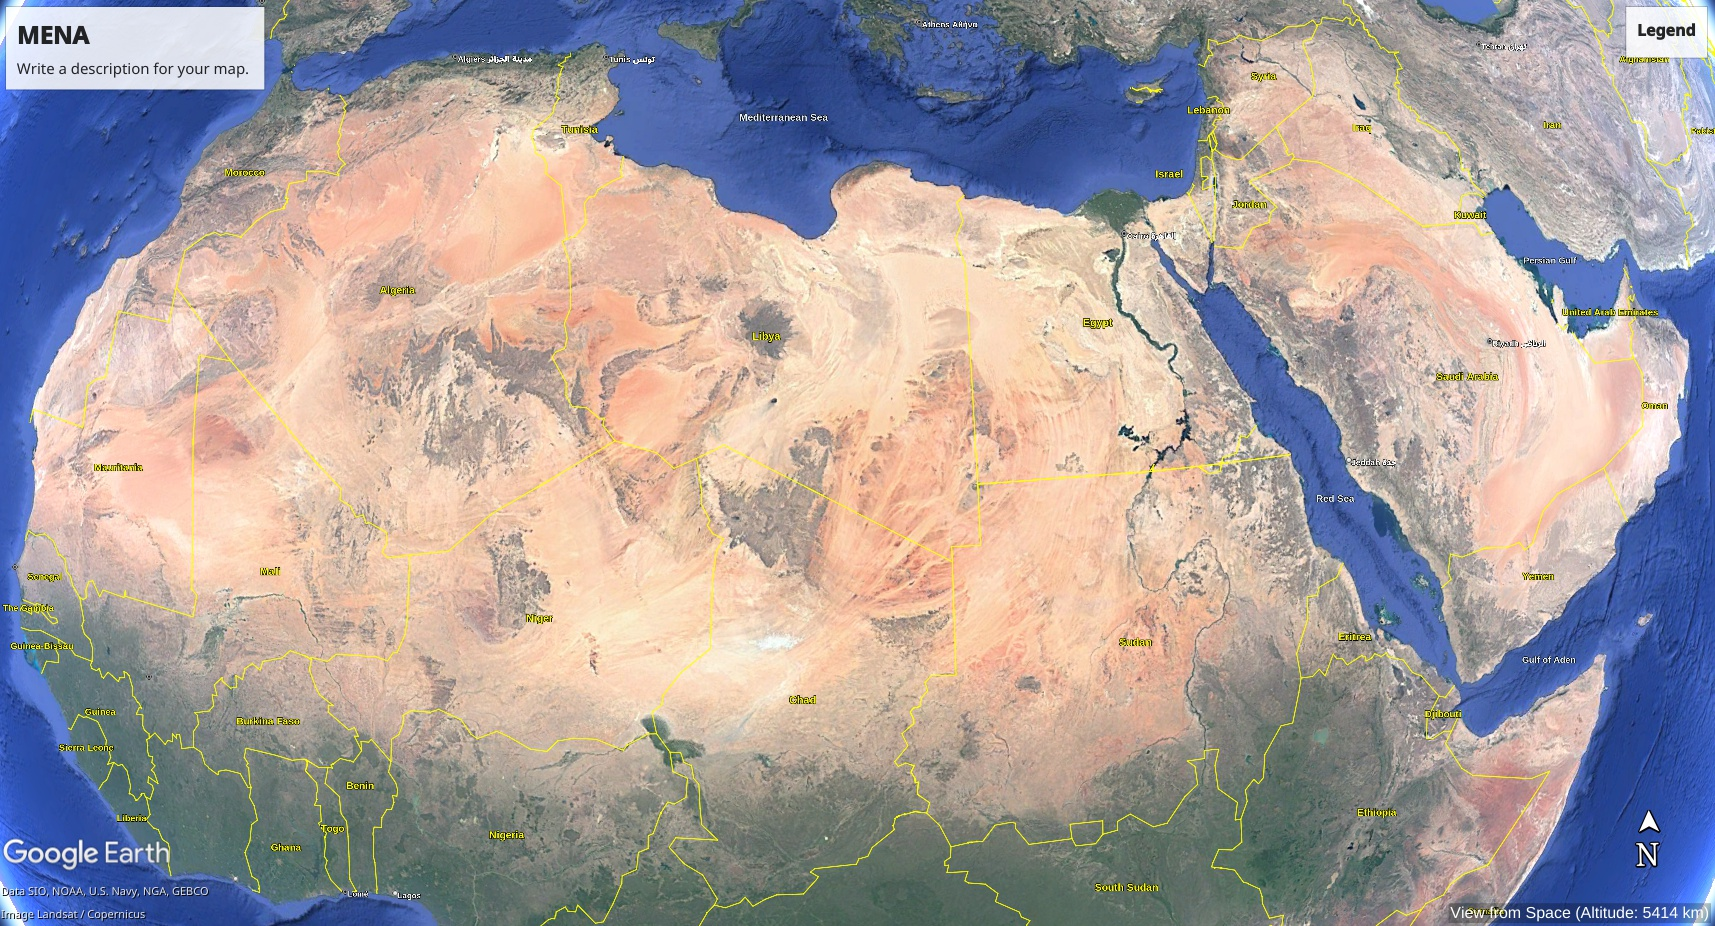
\includegraphics[width=0.75\linewidth]{mena.jpg}
    \caption{Mena}
    \label{fig:enter-label}
\end{figure}
\end{frame}
\begin{frame}{Zonne étudiée}
\framesubtitle{arabian peninsula }
\begin{figure}
    \centering
    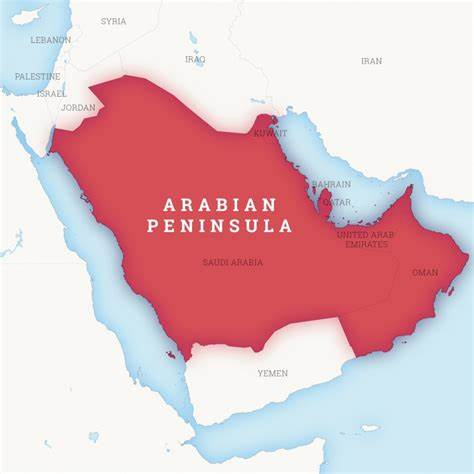
\includegraphics[width=0.75\linewidth]{arabian_peninsula.png}
    \caption{Focus on arabian peninsula}
    \label{fig:enter-label}
\end{figure}
\end{frame}
\begin{frame}{Zonne étudiée}
\framesubtitle{Afrique du nord}
\begin{figure}
    \centering
    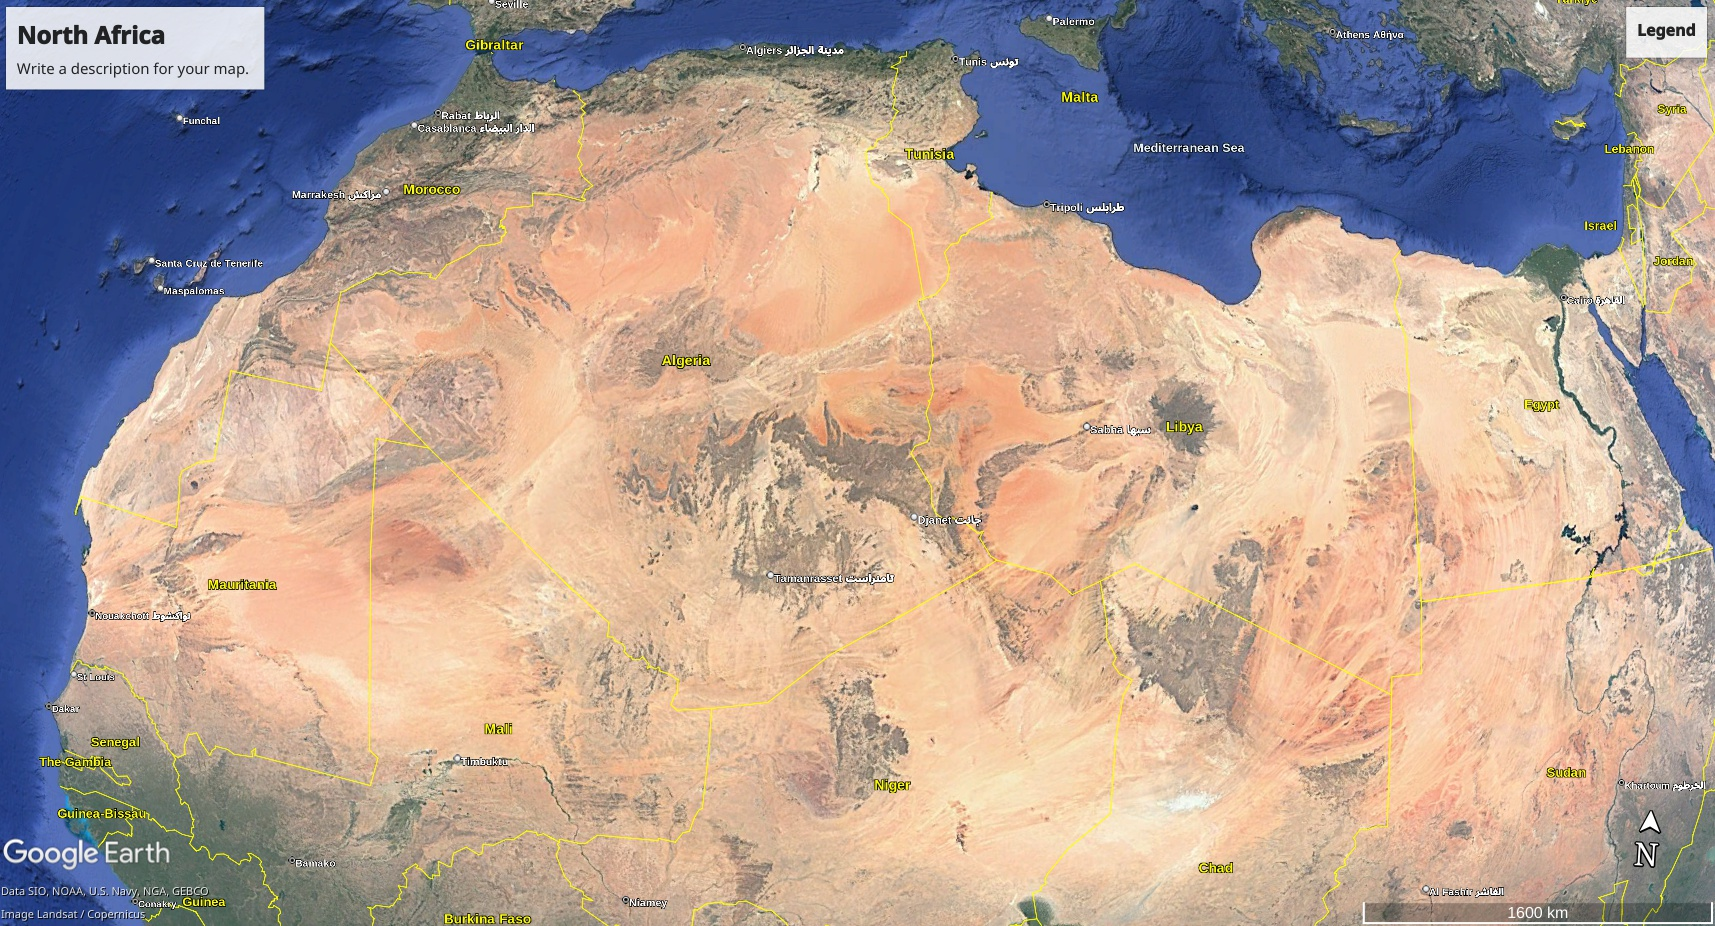
\includegraphics[width=0.75\linewidth]{north_africa.jpg}
    \caption{Afrique du nord}
    \label{fig:enter-label}
\end{figure}
\end{frame}
\subsection{Évaluation déterministe}

\begin{frame}{Concept}
  \textbf{Objectif :} Évaluer la précision des prévisions par rapport aux observations.
  \begin{itemize}
    \item \textbf{Anomaly Correlation Coefficient (ACC) :}
    
    \item \textbf{Root Mean Square Error (RMSE) :}
    
    \item \textbf{Coefficient de Détermination (R²) :}
   
  \end{itemize}
\end{frame}
\begin{frame}{Anomaly Correlation Coefficient (ACC)}
  \textbf{Formule :}
  \[
  ACC = \frac{\sum_{i=1}^N (P_i - \bar{P})(O_i - \bar{O})}{\sqrt{\sum_{i=1}^N (P_i - \bar{P})^2 \sum_{i=1}^N (O_i - \bar{O})^2}}
  \]
  \begin{itemize}
  \item \( N \) : Nombre total de données .
  \item \( P_i \) : Valeur prévue pour le \(i\)-ième point.
  \item \( O_i \) : Valeur observée pour le \(i\)-ième point.
  \item \( \bar{P} \) : Moyenne des valeurs prévues .
  \item \( \bar{O} \) : Moyenne des valeurs observées .
  
\end{itemize}

  \textbf{Interprétation :}
  \begin{itemize}
      \item Le \textbf{ACC} mesure la corrélation entre les anomalies prévues (\(P_i\)) et observées (\(O_i\)).

    \item Un score proche de 1 indique une excellente correspondance entre les prévisions et les observations.
  \end{itemize}
\end{frame}
\begin{frame}{Root Mean Square Error (RMSE)}
  \textbf{Formule :}
  \[
  RMSE = \sqrt{\frac{1}{N} \sum_{i=1}^N (P_i - O_i)^2}
  \]

 

  \textbf{Interprétation :}
  \begin{itemize}
    \item Le \textbf{RMSE} mesure les écarts quadratiques moyens entre les prévisions (\(P_i\)) et les observations (\(O_i\)).
    \item Une valeur faible indique un modèle performant avec de petites erreurs.
    \item Sensible aux erreurs extrêmes, ce qui le rend idéal pour identifier les grands écarts.
  \end{itemize}
\end{frame}
\begin{frame}{Coefficient de Détermination (R²)}
  \textbf{Formule :}
  \[
  R^2 = 1 - \frac{\sum_{i=1}^N (O_i - P_i)^2}{\sum_{i=1}^N (O_i - \bar{O})^2}
  \]

  \textbf{Interprétation :}
  \begin{itemize}
    \item Le \textbf{R²} représente la proportion de variance des observations (\(O_i\)) expliquée par les prévisions (\(P_i\)).
    \item Un R² proche de 1 indique une bonne performance du modèle.
    \item Si R² est négatif, le modèle est moins performant qu'une moyenne constante.
  \end{itemize}
\end{frame}
\subsection{Évaluation probabiliste}
\begin{frame}{Concept}
    \begin{block}{\textbf{Objectif}}
        Fournir une évaluation des performances d'un modèle en tenant compte de l'incertitude et en utilisant des distributions de probabilités. 
    \end{block}
    \begin{block}{\textbf{Catégories (Terciles)}}
        \begin{itemize}
            \item \textbf{En dessous de la moyenne} : Inférieur au premier tiers (1/3).
            \item \textbf{Proche de la moyenne} : Entre 1/3 et 2/3.
            \item \textbf{Au-dessus de la moyenne} : Supérieur au dernier tiers (2/3).
        \end{itemize}
    \end{block}
\end{frame}
\begin{frame}{Les métriques probabilistiques évaluent: }
\begin{block}
\centering
\renewcommand{\arraystretch}{1.4} % Espacement vertical
\setlength{\tabcolsep}{8pt} % Espacement horizontal
\resizebox{\textwidth}{!}{%
\begin{tabular}{|>{\columncolor{subtitlecolor}\color{white}}p{4.5cm}|p{7.5cm}|p{5.5cm}|}
\hline
\rowcolor{titlecolor} \color{white} \textbf{Concept} & \color{white} \textbf{Définition} & \color{white} \textbf{Métriques Associées} \\
\hline
\textbf{Fiabilité} & Cohérence entre les probabilités prédites et les observations, reflétant la capacité du modèle à produire des prévisions fiables. & Brier Score (BS), Calibration, Diagramme de Fiabilité \\
\hline
\textbf{Résolution} & Capacité du modèle à différencier les diverses situations climatiques en prédisant des probabilités variées selon les scénarios. & Brier Score (BS), Ranked Probability Score (RPS) \\
\hline
\textbf{Discrimination} & Aptitude du modèle à distinguer correctement les événements observés (succès) des non-événements (échecs). & Receiver Operating Characteristic (ROC), Area Under Curve (AUC), Accuracy (ACC) \\
\hline
\end{tabular}%
}
\end{block}
\end{frame}

\begin{frame}{Brier Score}
  \textbf{Formule :}
  \[
  BS = \frac{1}{N} \sum_{i=1}^N (P_i - O_i)^2
  \]
  \begin{itemize}
  \item \( N \) : Nombre total de points de données.
  \item \( P_i \) : Probabilité prévue pour le \(i\)-ième point.
  \item \( O_i \) : Valeur observée pour le \(i\)-ième point (0 ou 1).
  \end{itemize}
  
  \textbf{Interprétation :}
  \begin{itemize}
      \item Le \textbf{Brier Score} mesure l'erreur quadratique moyenne entre les probabilités prévues et les résultats observés.
      \item Un score de Brier faible indique une meilleure précision des prévisions probabilistes.
  \end{itemize}
\end{frame}
\begin{frame}{Fiabilité (Reliability)}
  \textbf{Formule :}
  \[
  \text{Fiabilité} = \frac{1}{N} \sum_{i=1}^N \left| P_i - O_i \right|
  \]
  \begin{itemize}
  \item \( N \) : Nombre total de données.
  \item \( P_i \) : Probabilité prévue pour le \(i\)-ième point.
  \item \( O_i \) : Résultat observé pour le \(i\)-ième point (0 ou 1).
  \end{itemize}
  
  \textbf{Interprétation :}
  \begin{itemize}
      \item La \textbf{fiabilité} mesure l'écart entre la probabilité prévue et la fréquence réelle des événements observés.
      \item Une bonne fiabilité signifie que les probabilités prévues correspondent bien aux fréquences observées.
  \end{itemize}
\end{frame}

\begin{frame}{Ranked Probability Score (RPS)}
  \textbf{Formule :}
  \[
  RPS = \sum_{i=1}^N \left( \sum_{j=1}^M (P_{i,j} - O_{i,j})^2 \right)
  \]
  \begin{itemize}
  \item \( N \) : Nombre total de points de données.
  \item \( M \) : Nombre de catégories possibles.
  \item \( P_{i,j} \) : Probabilité prévue pour la catégorie \(j\)-ième pour le \(i\)-ième point.
  \item \( O_{i,j} \) : Indicateur binaire (0 ou 1) pour la catégorie \(j\)-ième du \(i\)-ième point observé.
  \end{itemize}
  
  \textbf{Interprétation :}
  \begin{itemize}
      \item Le \textbf{RPS} mesure la différence entre les prévisions classées et les résultats observés, en prenant en compte toutes les catégories.
      \item Un RPS faible indique une meilleure correspondance entre les prévisions classées et les observations.
  \end{itemize}
\end{frame}
\begin{frame}{Receiver Operating Characteristic (ROC)}
  \textbf{Formule :}
  \[
  \text{AUC} = \int_0^1 \text{True Positive Rate}(x) \, \text{False Positive Rate}(x) \, dx
  \]
  \begin{itemize}
  \item Taux de vrais positifs (TPR) : \( \text{TPR} = \frac{TP}{TP + FN} \)
  \item Taux de faux positifs (FPR) : \( \text{FPR} = \frac{FP}{FP + TN} \)
  \item L'aire sous la courbe (AUC) mesure la performance du classificateur à distinguer les classes.
  \end{itemize}
  
  \textbf{Interprétation :}
  \begin{itemize}
      \item Une AUC de 1 indique une parfaite séparation entre les classes positives et négatives.
      \item Une AUC de 0.5 indique une performance équivalente à un tirage au sort.
  \end{itemize}
\end{frame}
\begin{frame}{Relative Operating Characteristic Score (ROCSS)}
  \textbf{Formule :}
  \[
  \text{ROCSS} = \frac{\text{AUC} - \text{AUC}\text{random}}{1 - \text{AUC}\text{random}}
  \]
  \begin{itemize}
  \item \text{AUC} : Aire sous la courbe ROC pour le modèle testé.
  \item \text{AUC}\_\text{random} : AUC pour un modèle aléatoire (généralement 0.5).
  \end{itemize}
  
  \textbf{Interprétation :}
  \begin{itemize}
      \item La \textbf{ROCSS} donne une évaluation de la performance relative du modèle par rapport à un modèle aléatoire.
      \item Un score plus élevé indique une meilleure performance du modèle par rapport au hasard.
  \end{itemize}
\end{frame}
\begin{frame}{Température}
\framesubtitle{Déterministe - ACC}

\section{Evaluation de la Température}
\subsection{Evaluation Déterministe}
\begin{figure}
    \centering
    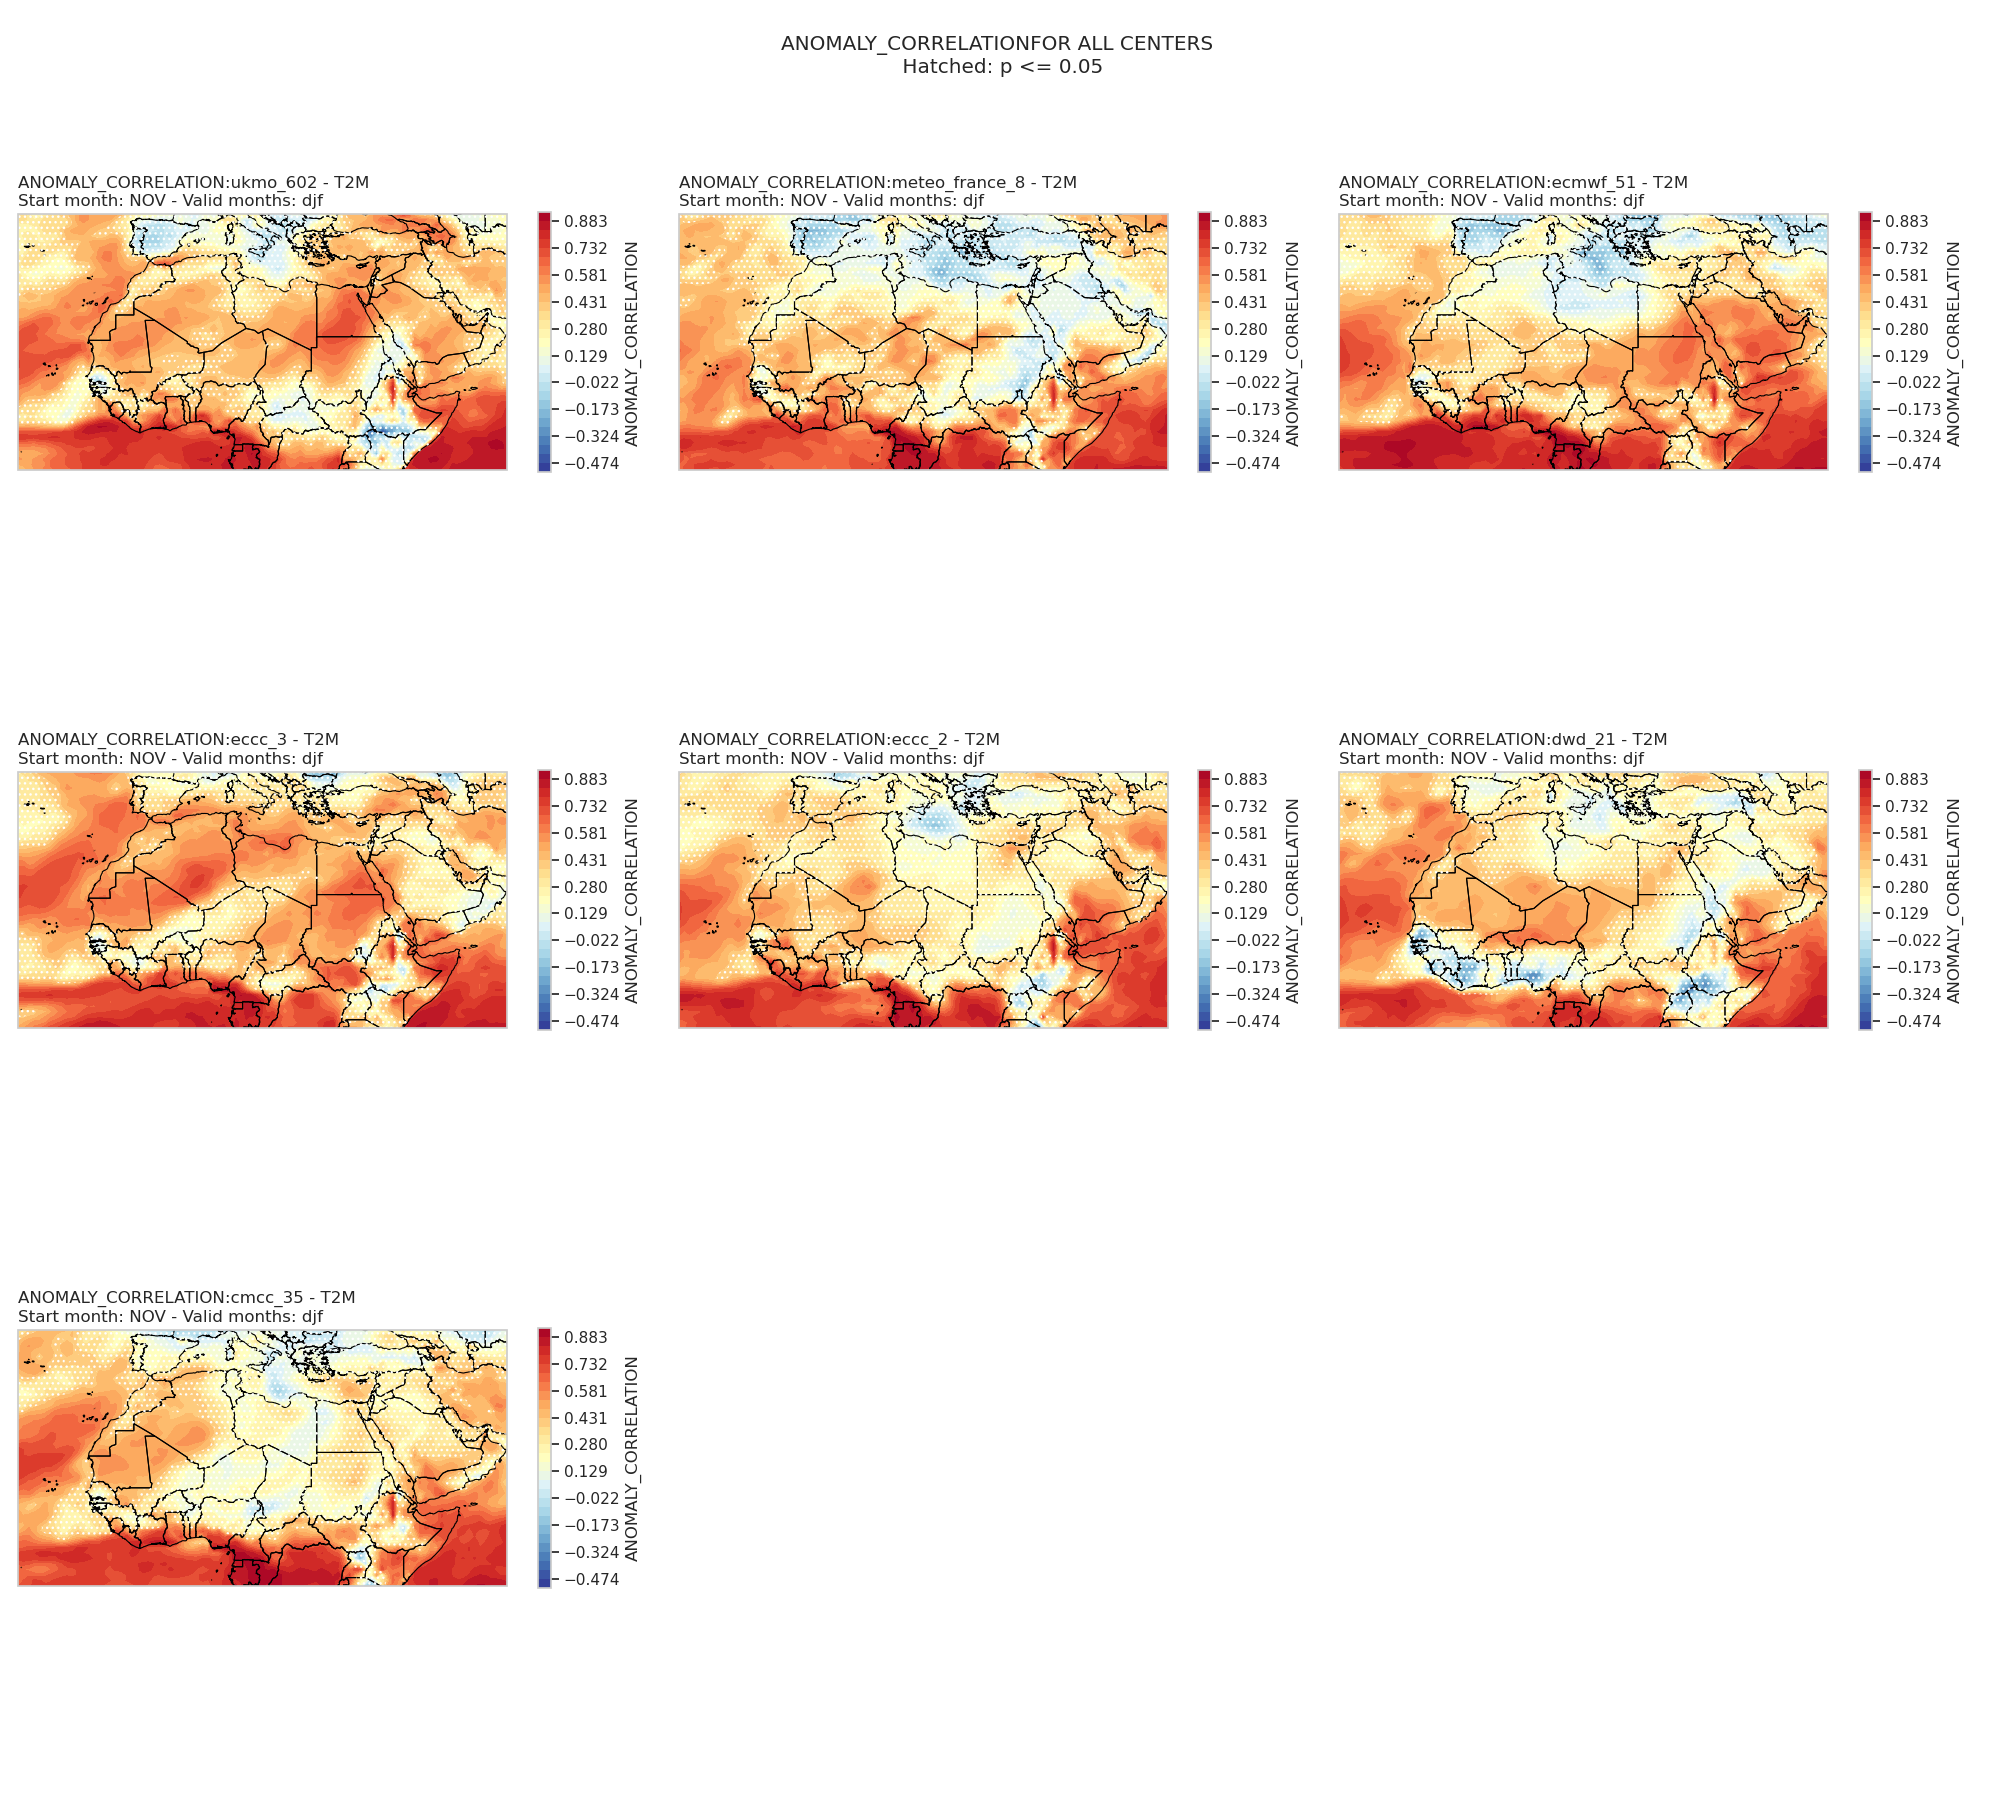
\includegraphics[width=0.7\linewidth]{/home/mohamed/EHTPIII/MODELISATION/Report_25_11/plots/det/acc/ANOMALY_CORRELATION_djf_t2m.png}
    \caption{ACC pour la température - DJF  }
    \label{fig:enter-label}
\end{figure}
\end{frame}

\begin{frame}{Température}
\framesubtitle{Déterministe - ACC}

\begin{figure}
    \centering
    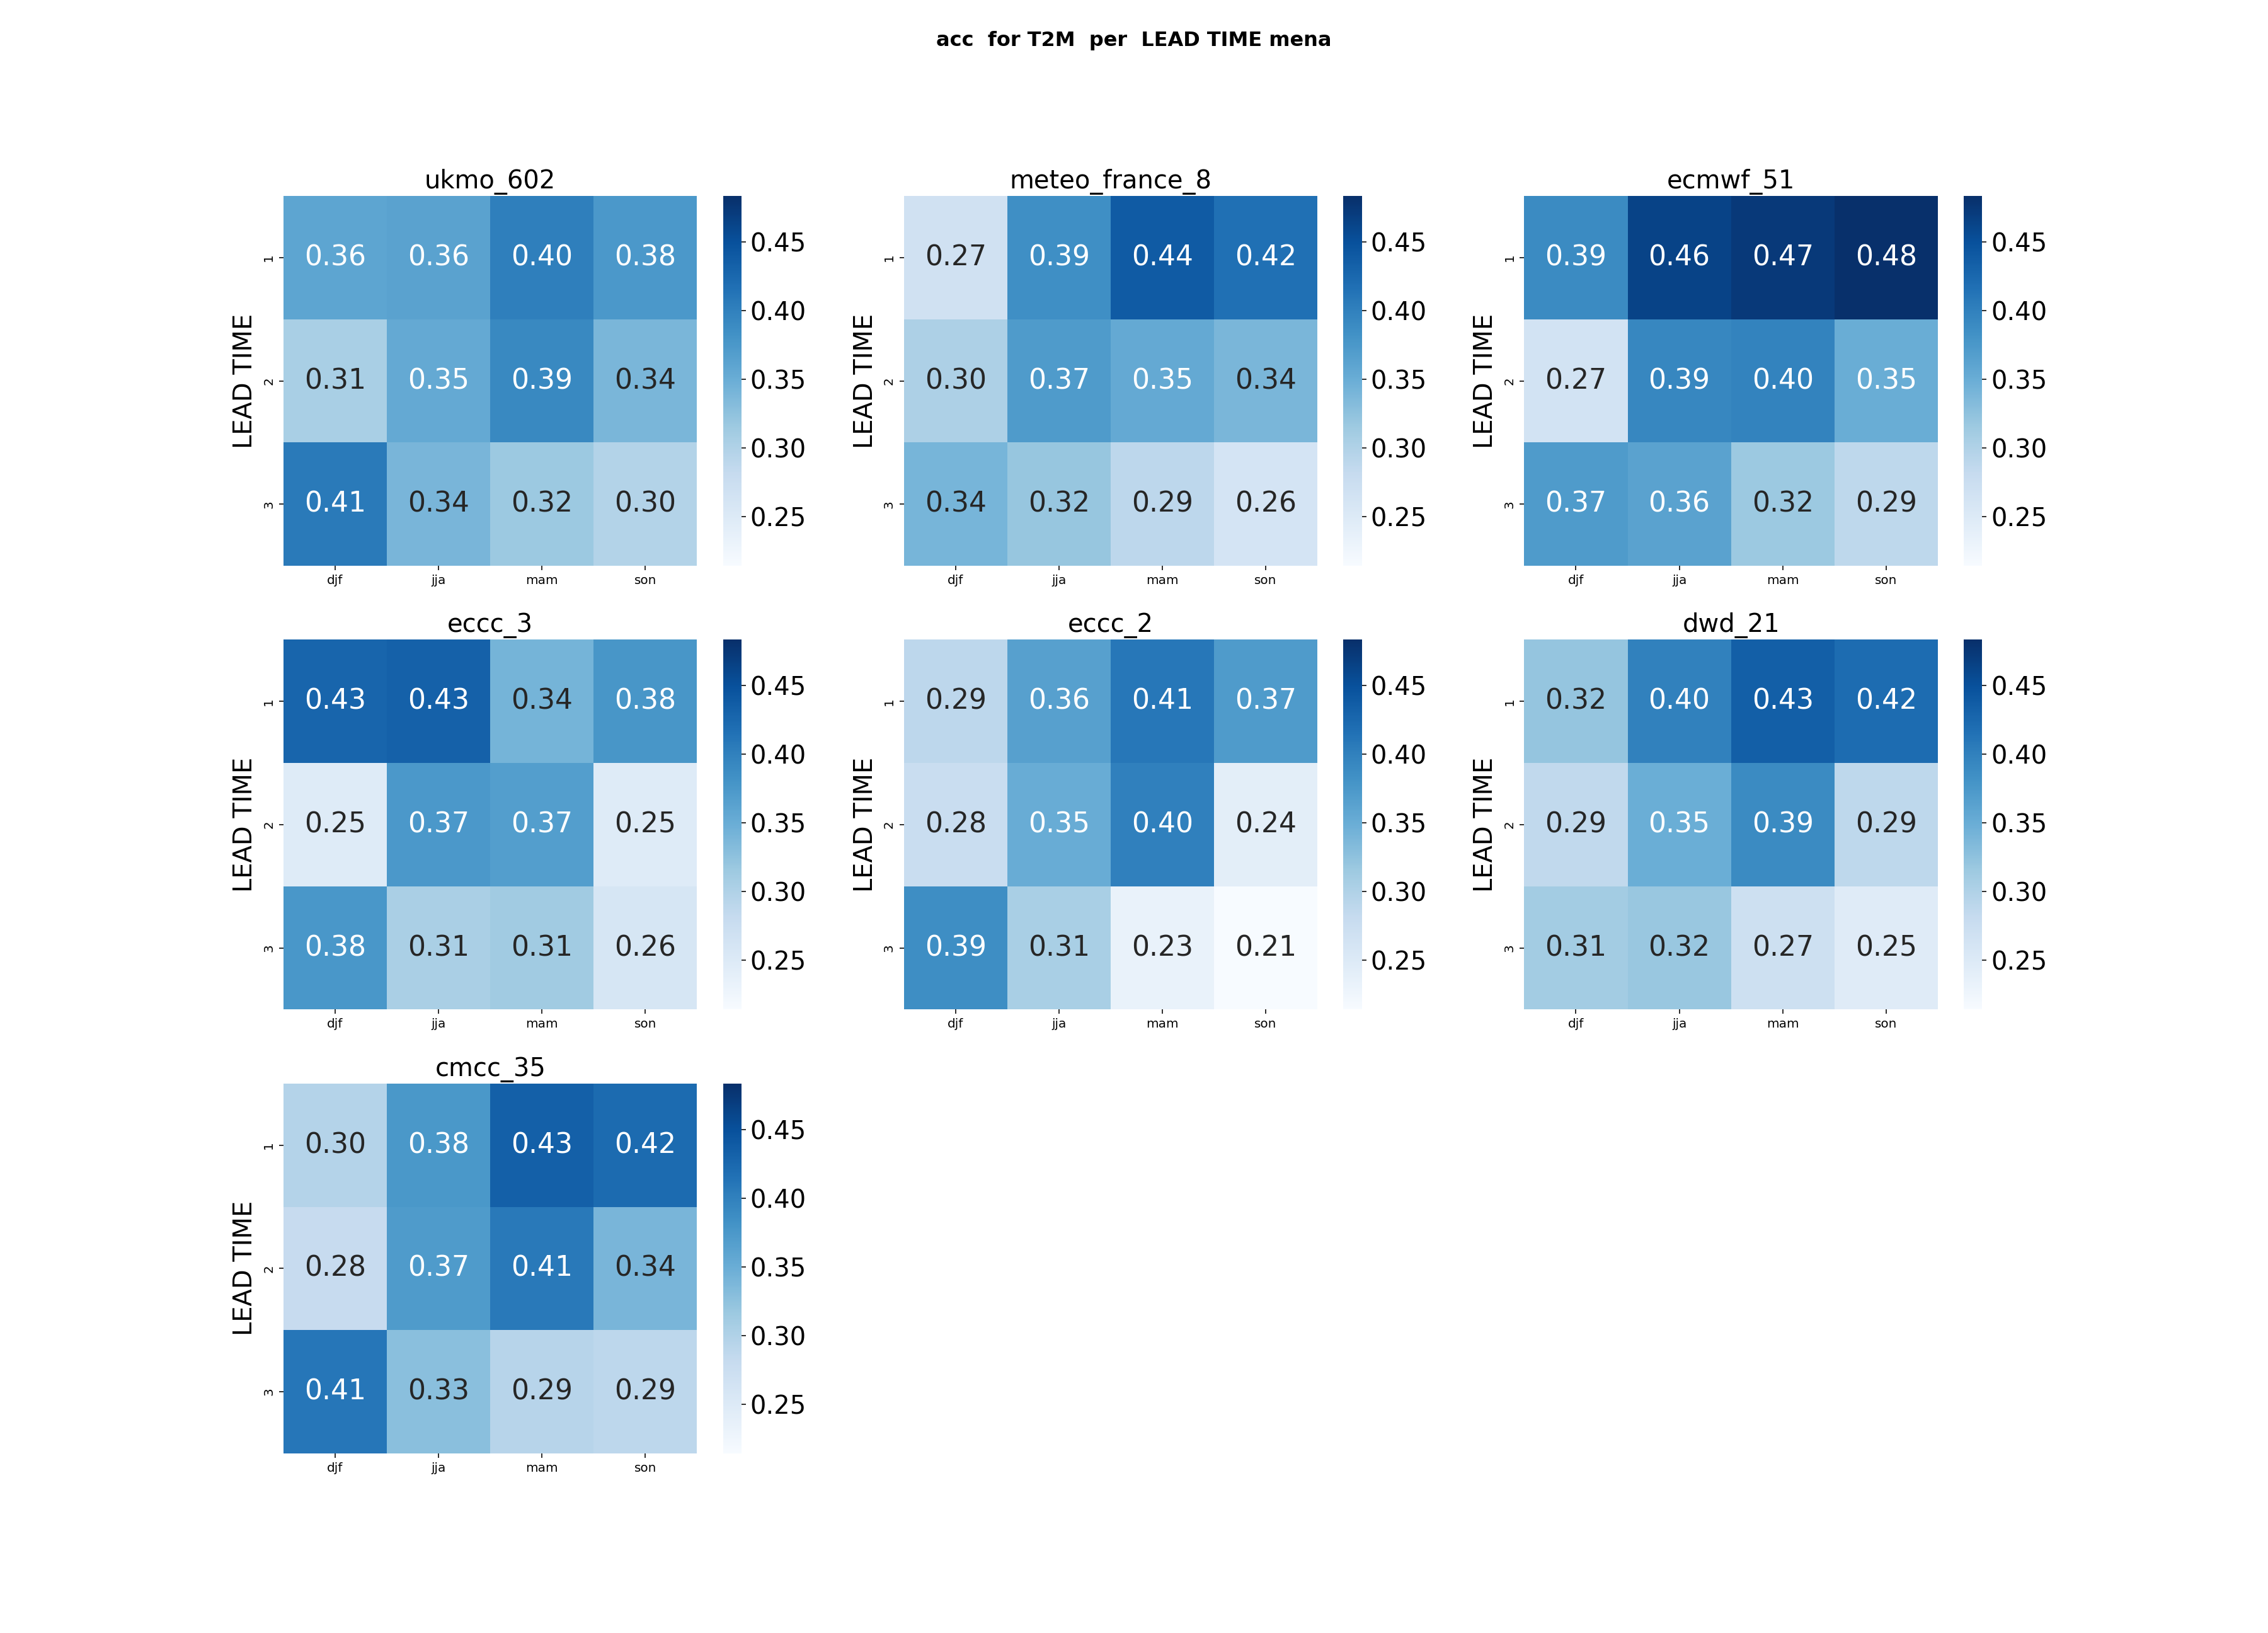
\includegraphics[width=0.8\linewidth]{/home/mohamed/EHTPIII/MODELISATION/Report_25_11/plots/det/acc/acc_T2M_mena.png}
    \caption{Heatmap ACC pour la température }
    \label{fig:enter-label}
\end{figure}
\end{frame}

\begin{frame}{Température}
\framesubtitle{Déterministe - RMSE}

\begin{figure}
    \centering
    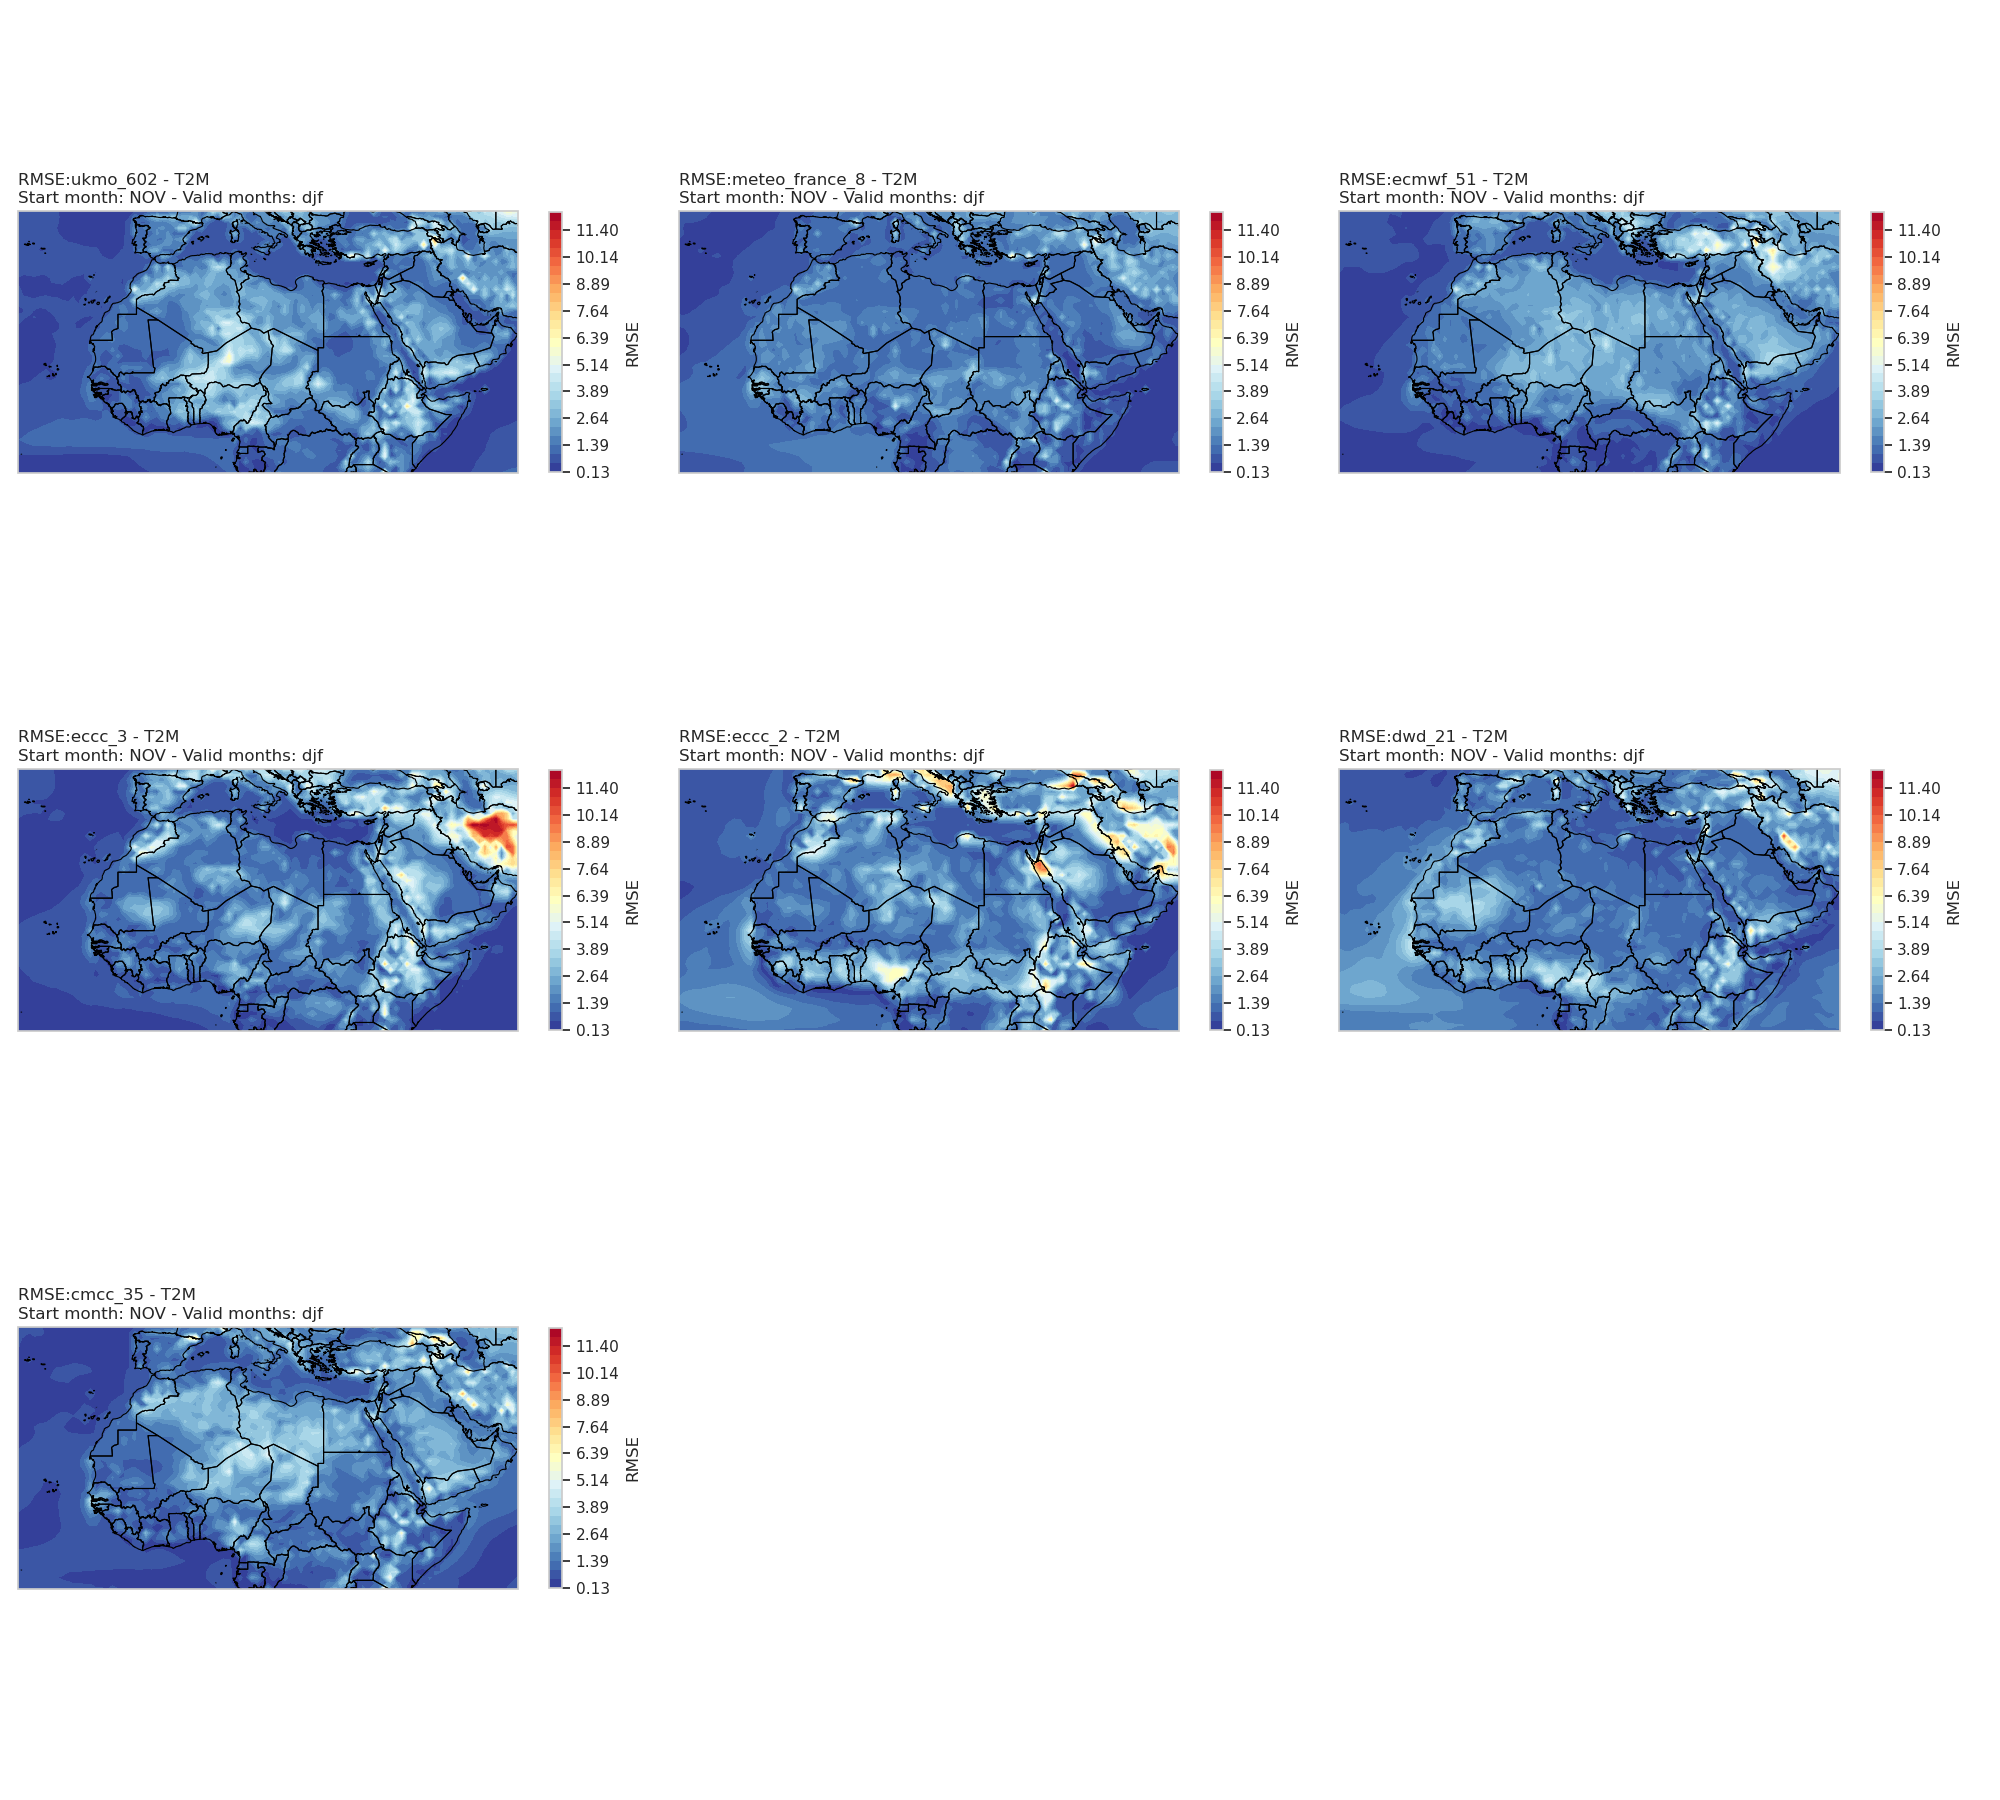
\includegraphics[width=0.7\linewidth]{/home/mohamed/EHTPIII/MODELISATION/Report_25_11/plots/det/rmse/rmse_djf_t2m.png}
    \caption{RMSE pour la température - DJF  }
    \label{fig:enter-label}
\end{figure}
\end{frame}

\begin{frame}{température}
\framesubtitle{Déterministe - RMSE}

\begin{figure}
    \centering 
    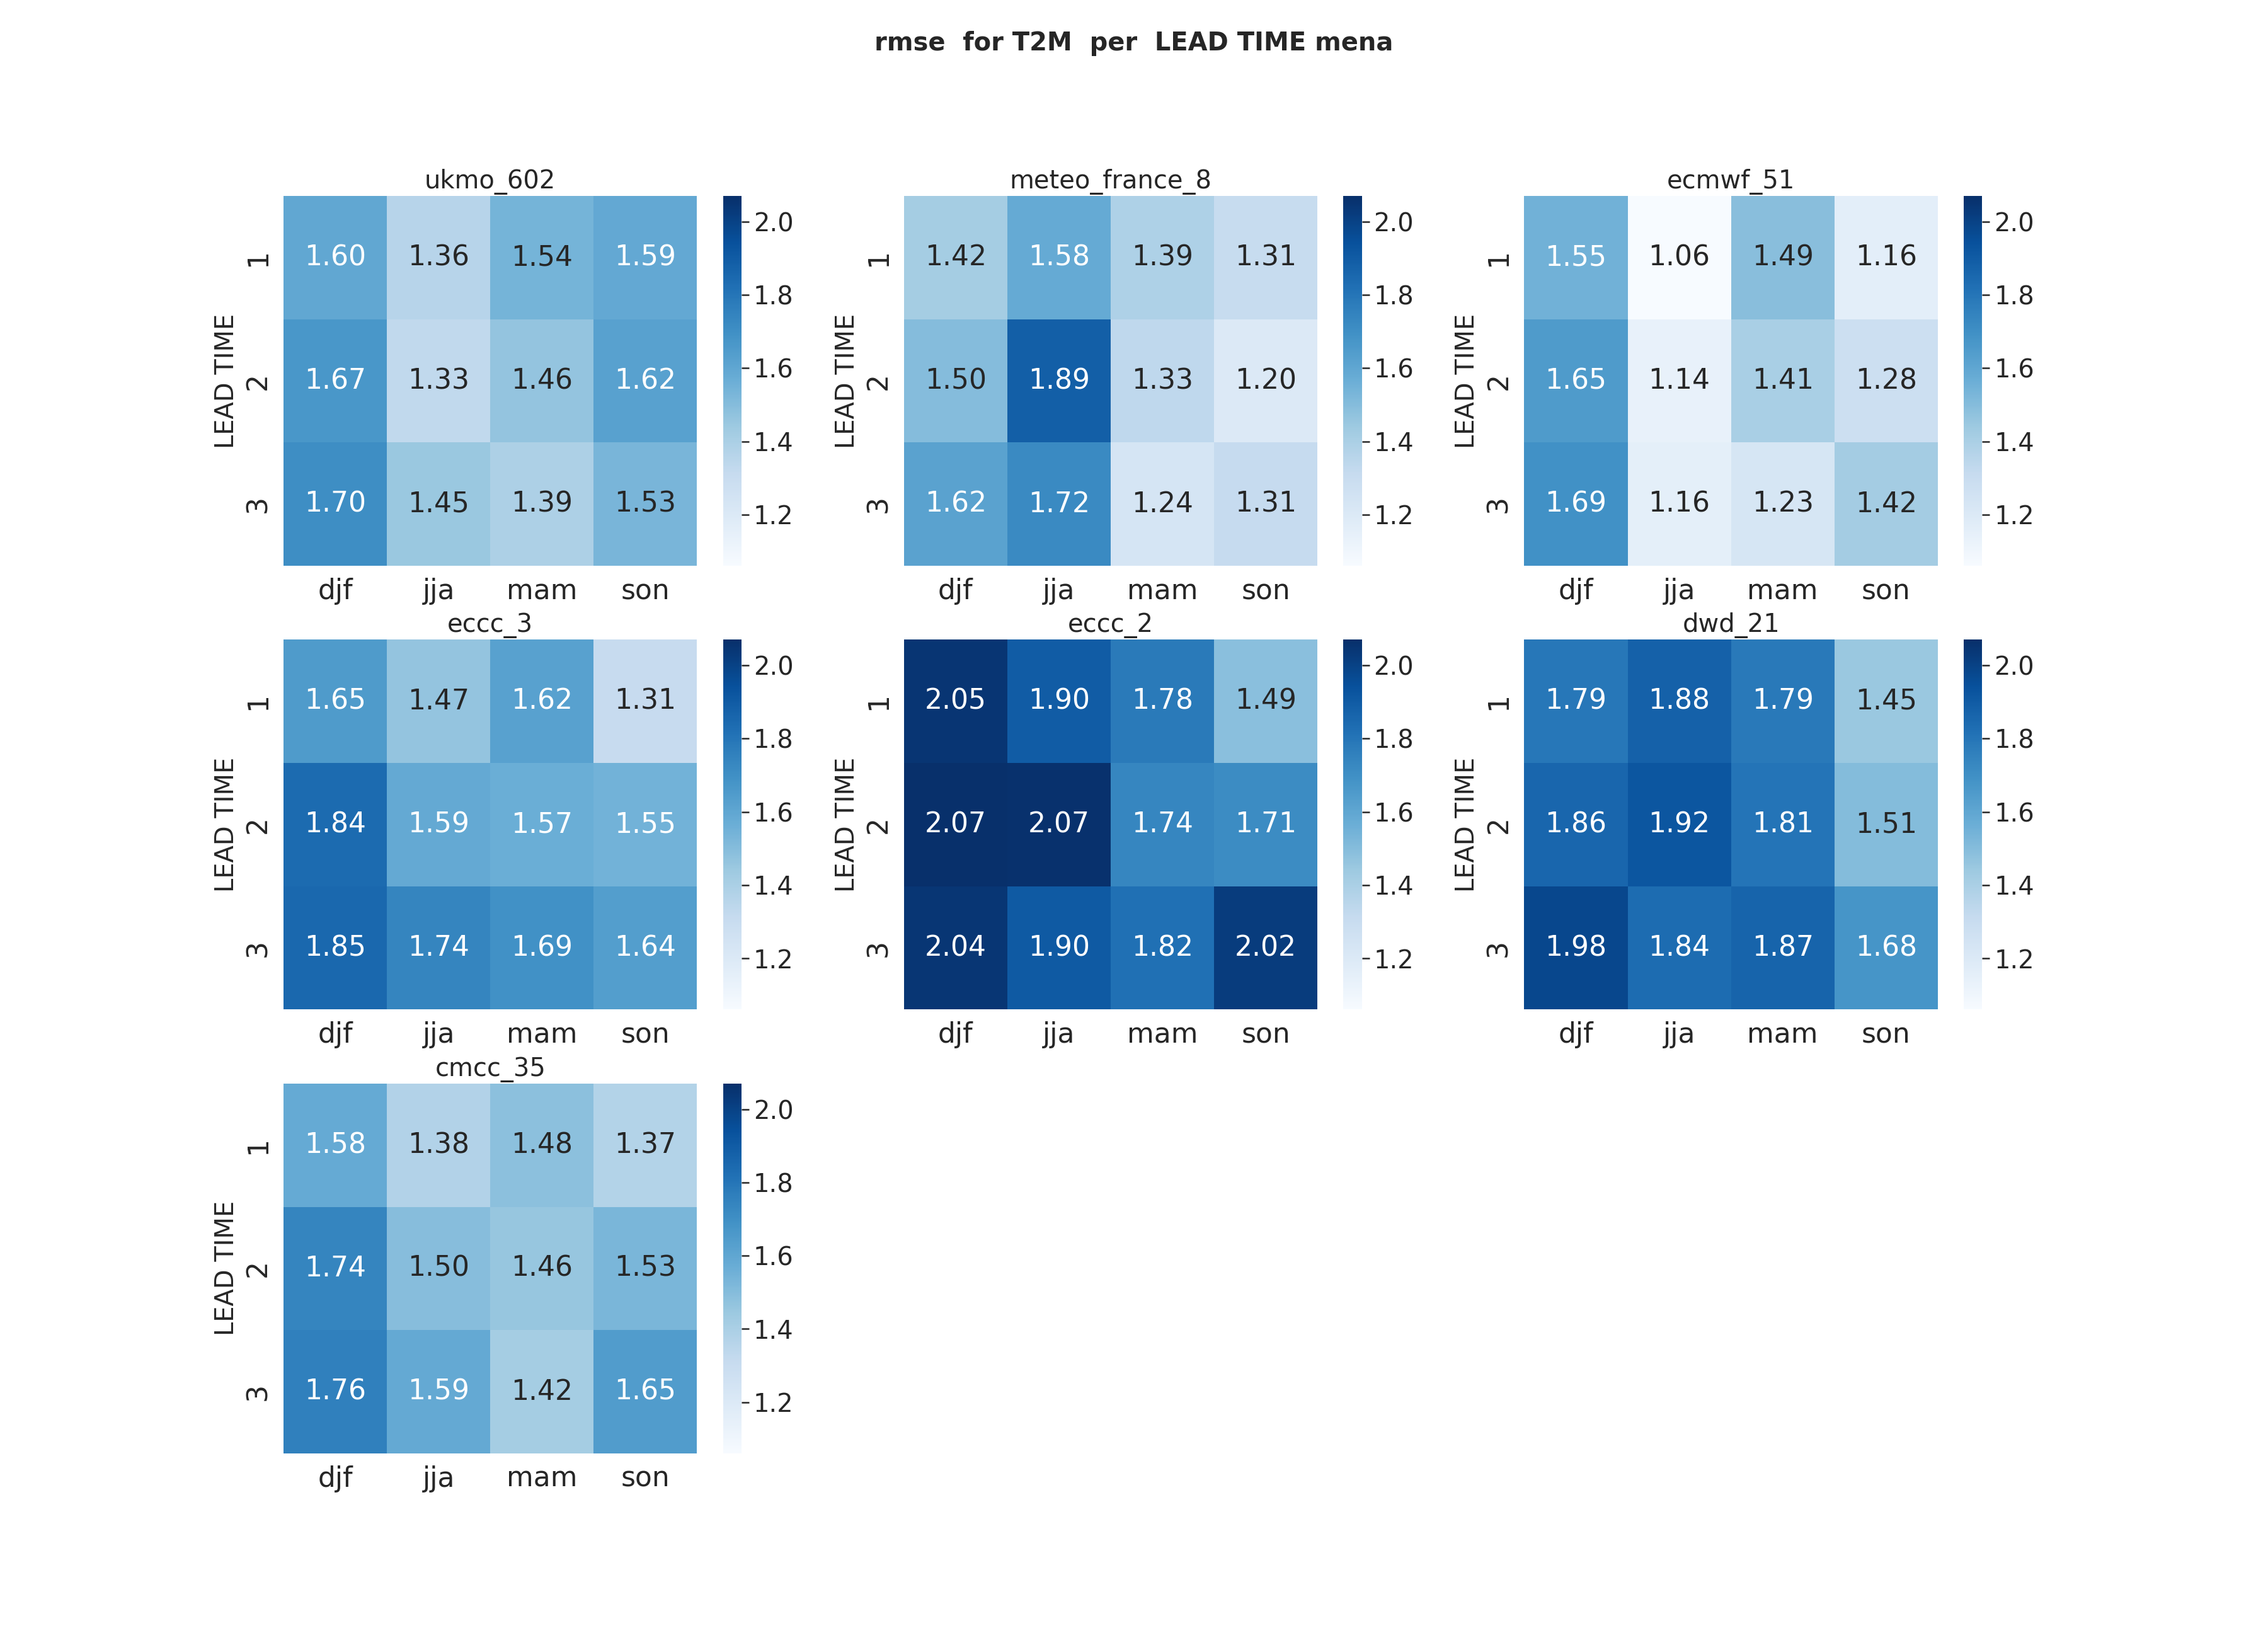
\includegraphics[width=0.8\linewidth]{/home/mohamed/EHTPIII/MODELISATION/Report_25_11/plots/det/rmse/rmse_T2M_mena.png}
    \caption{Heatmap RMSE pour la température  }
    \label{fig:enter-label}
\end{figure}
\end{frame}

\subsection{Evaluation Probabiliste}

\begin{frame}{Température}
\framesubtitle{Probabiliste - BS (0 pour un BS meilleur)}

\begin{figure}
    \centering
    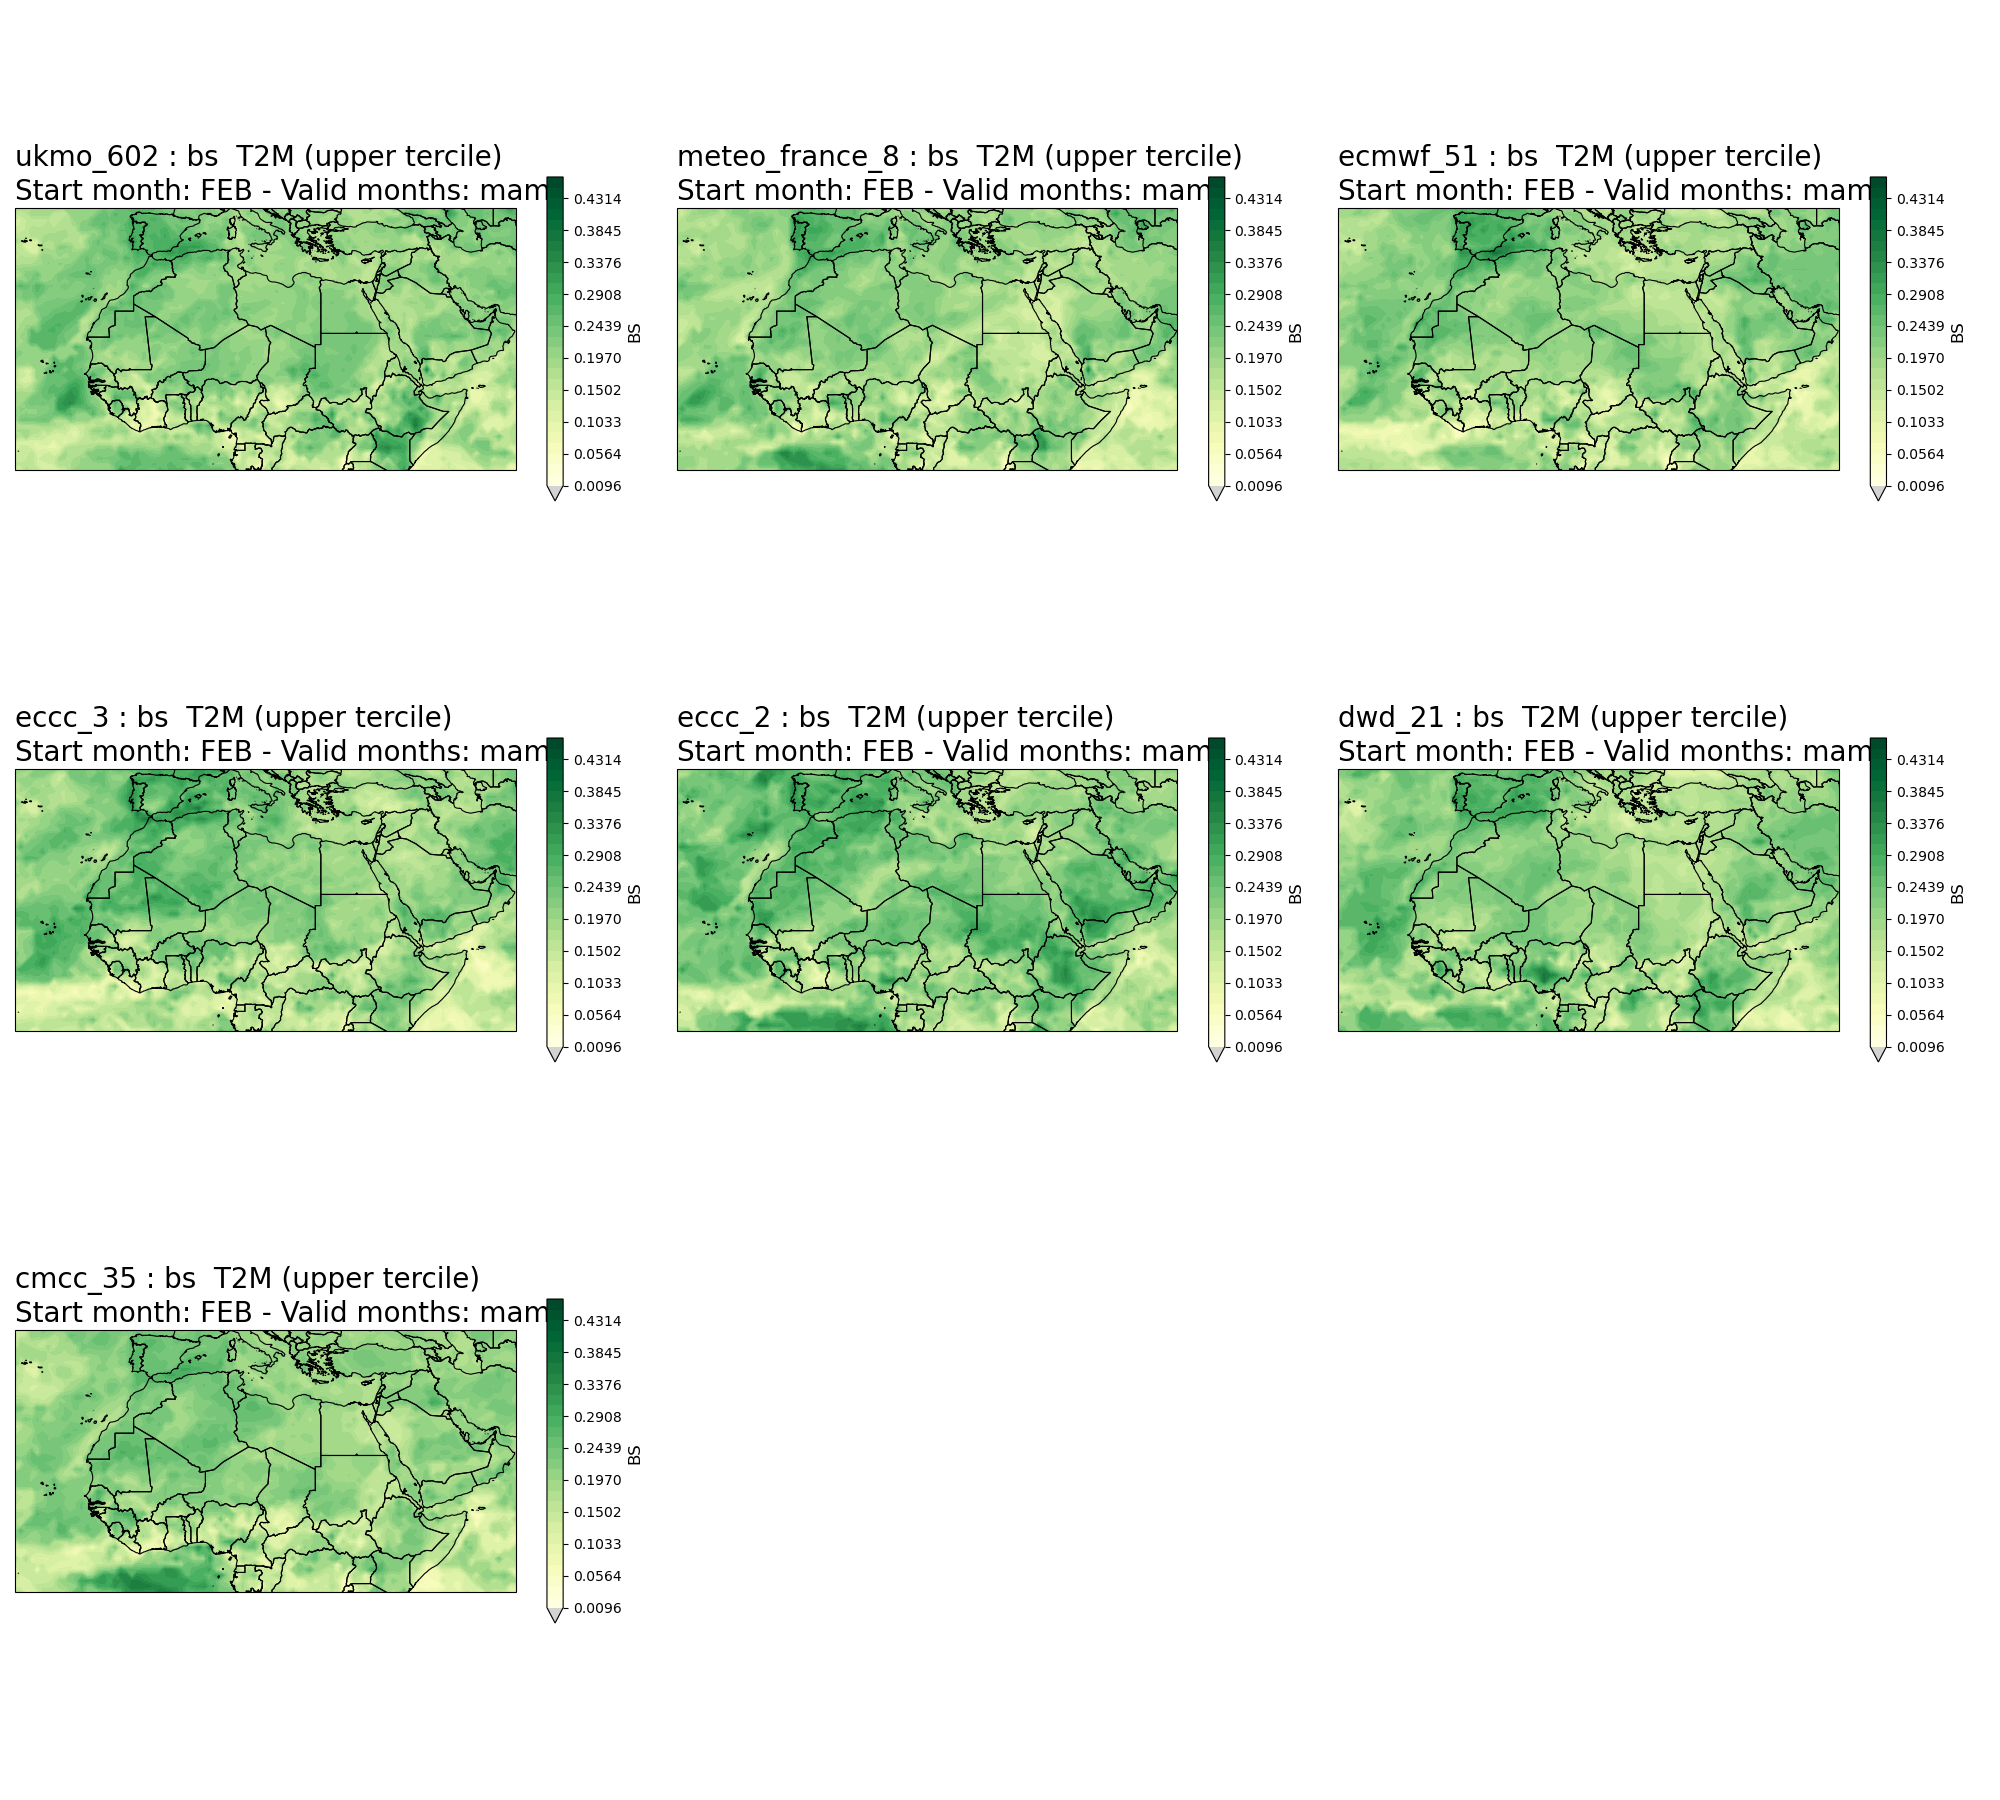
\includegraphics[width=0.7\linewidth]{/home/mohamed/EHTPIII/MODELISATION/Report_25_11/plots/prob/bs/bs_mam_upper_t2m.png}
    \caption{BS pour la température - MAM  Upper Tercile }
    \label{fig:enter-label}
\end{figure}
\end{frame}

\begin{frame}{Température}
\framesubtitle{Probabiliste - BS (0 pour un BS meilleur)}

\begin{figure}
    \centering
    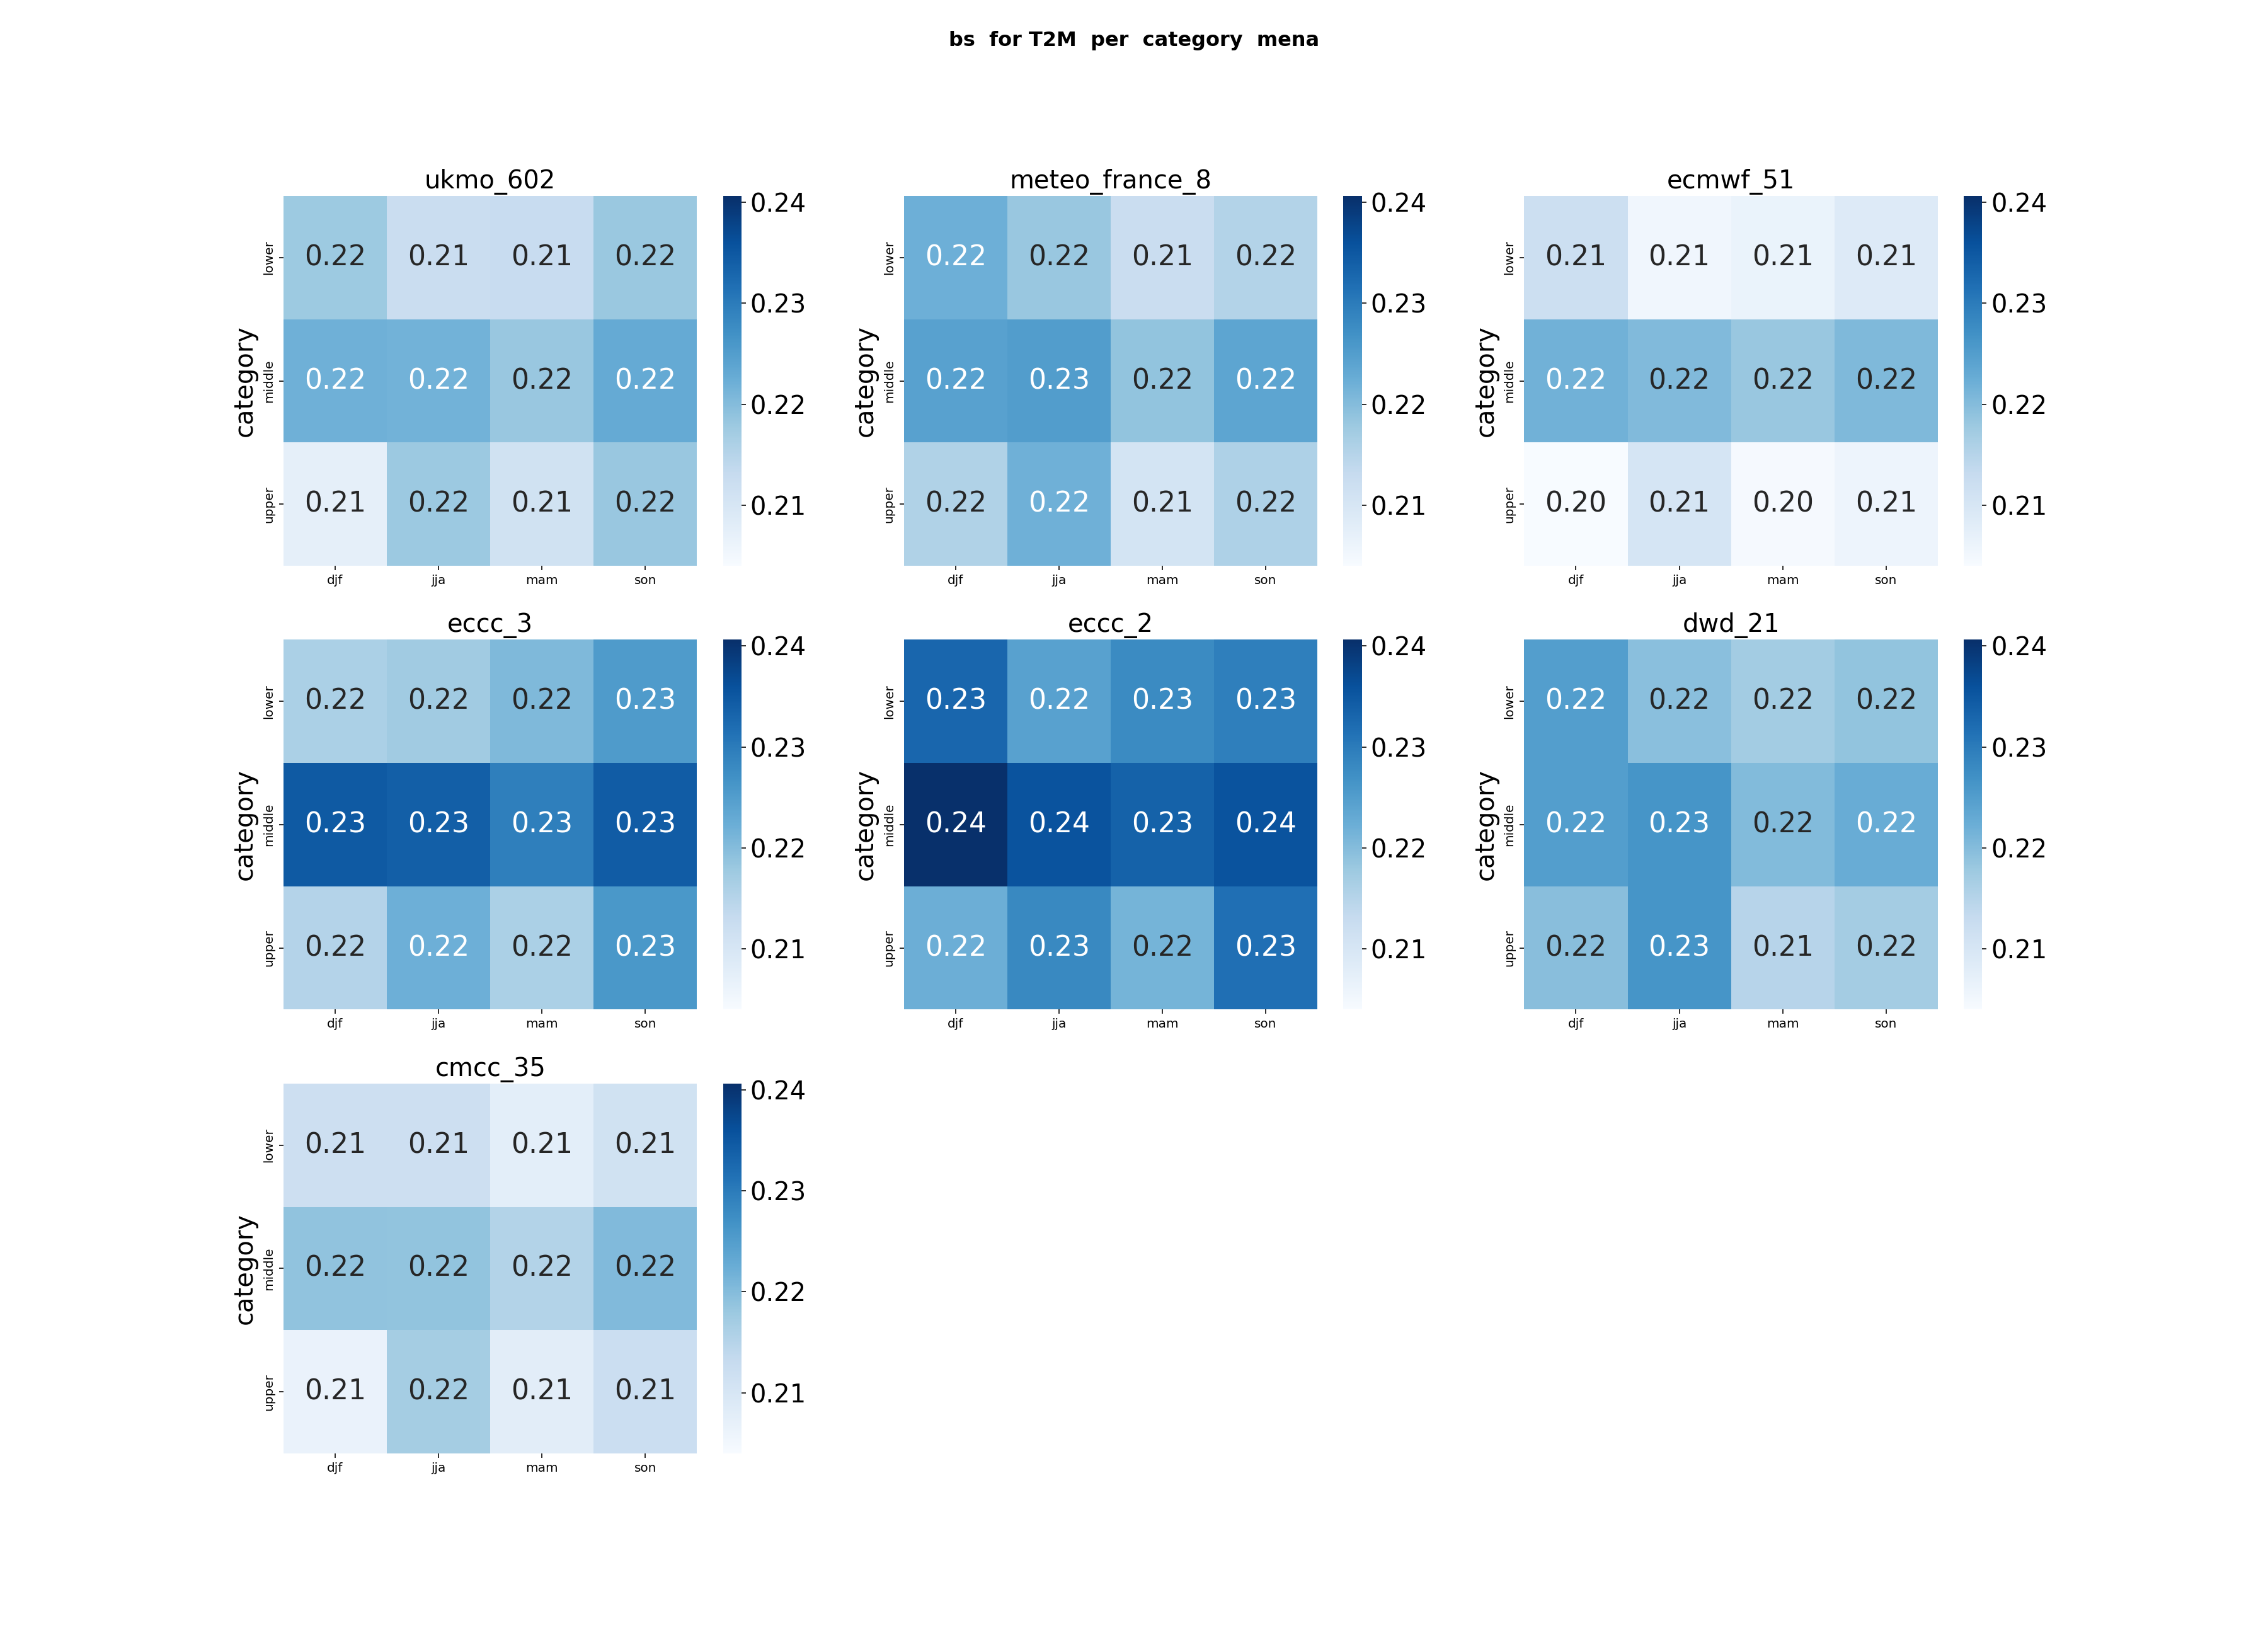
\includegraphics[width=0.8\linewidth]{/home/mohamed/EHTPIII/MODELISATION/Report_25_11/plots/prob/bs/bs_T2M_category_mena.png}
    \caption{Heatmap BS par Catégorie.  }
    \label{fig:enter-label}
\end{figure}
\end{frame}


\begin{frame}{Température}
\framesubtitle{Probabiliste - BS (0 pour un BS meilleur)}

\begin{figure}
    \centering
    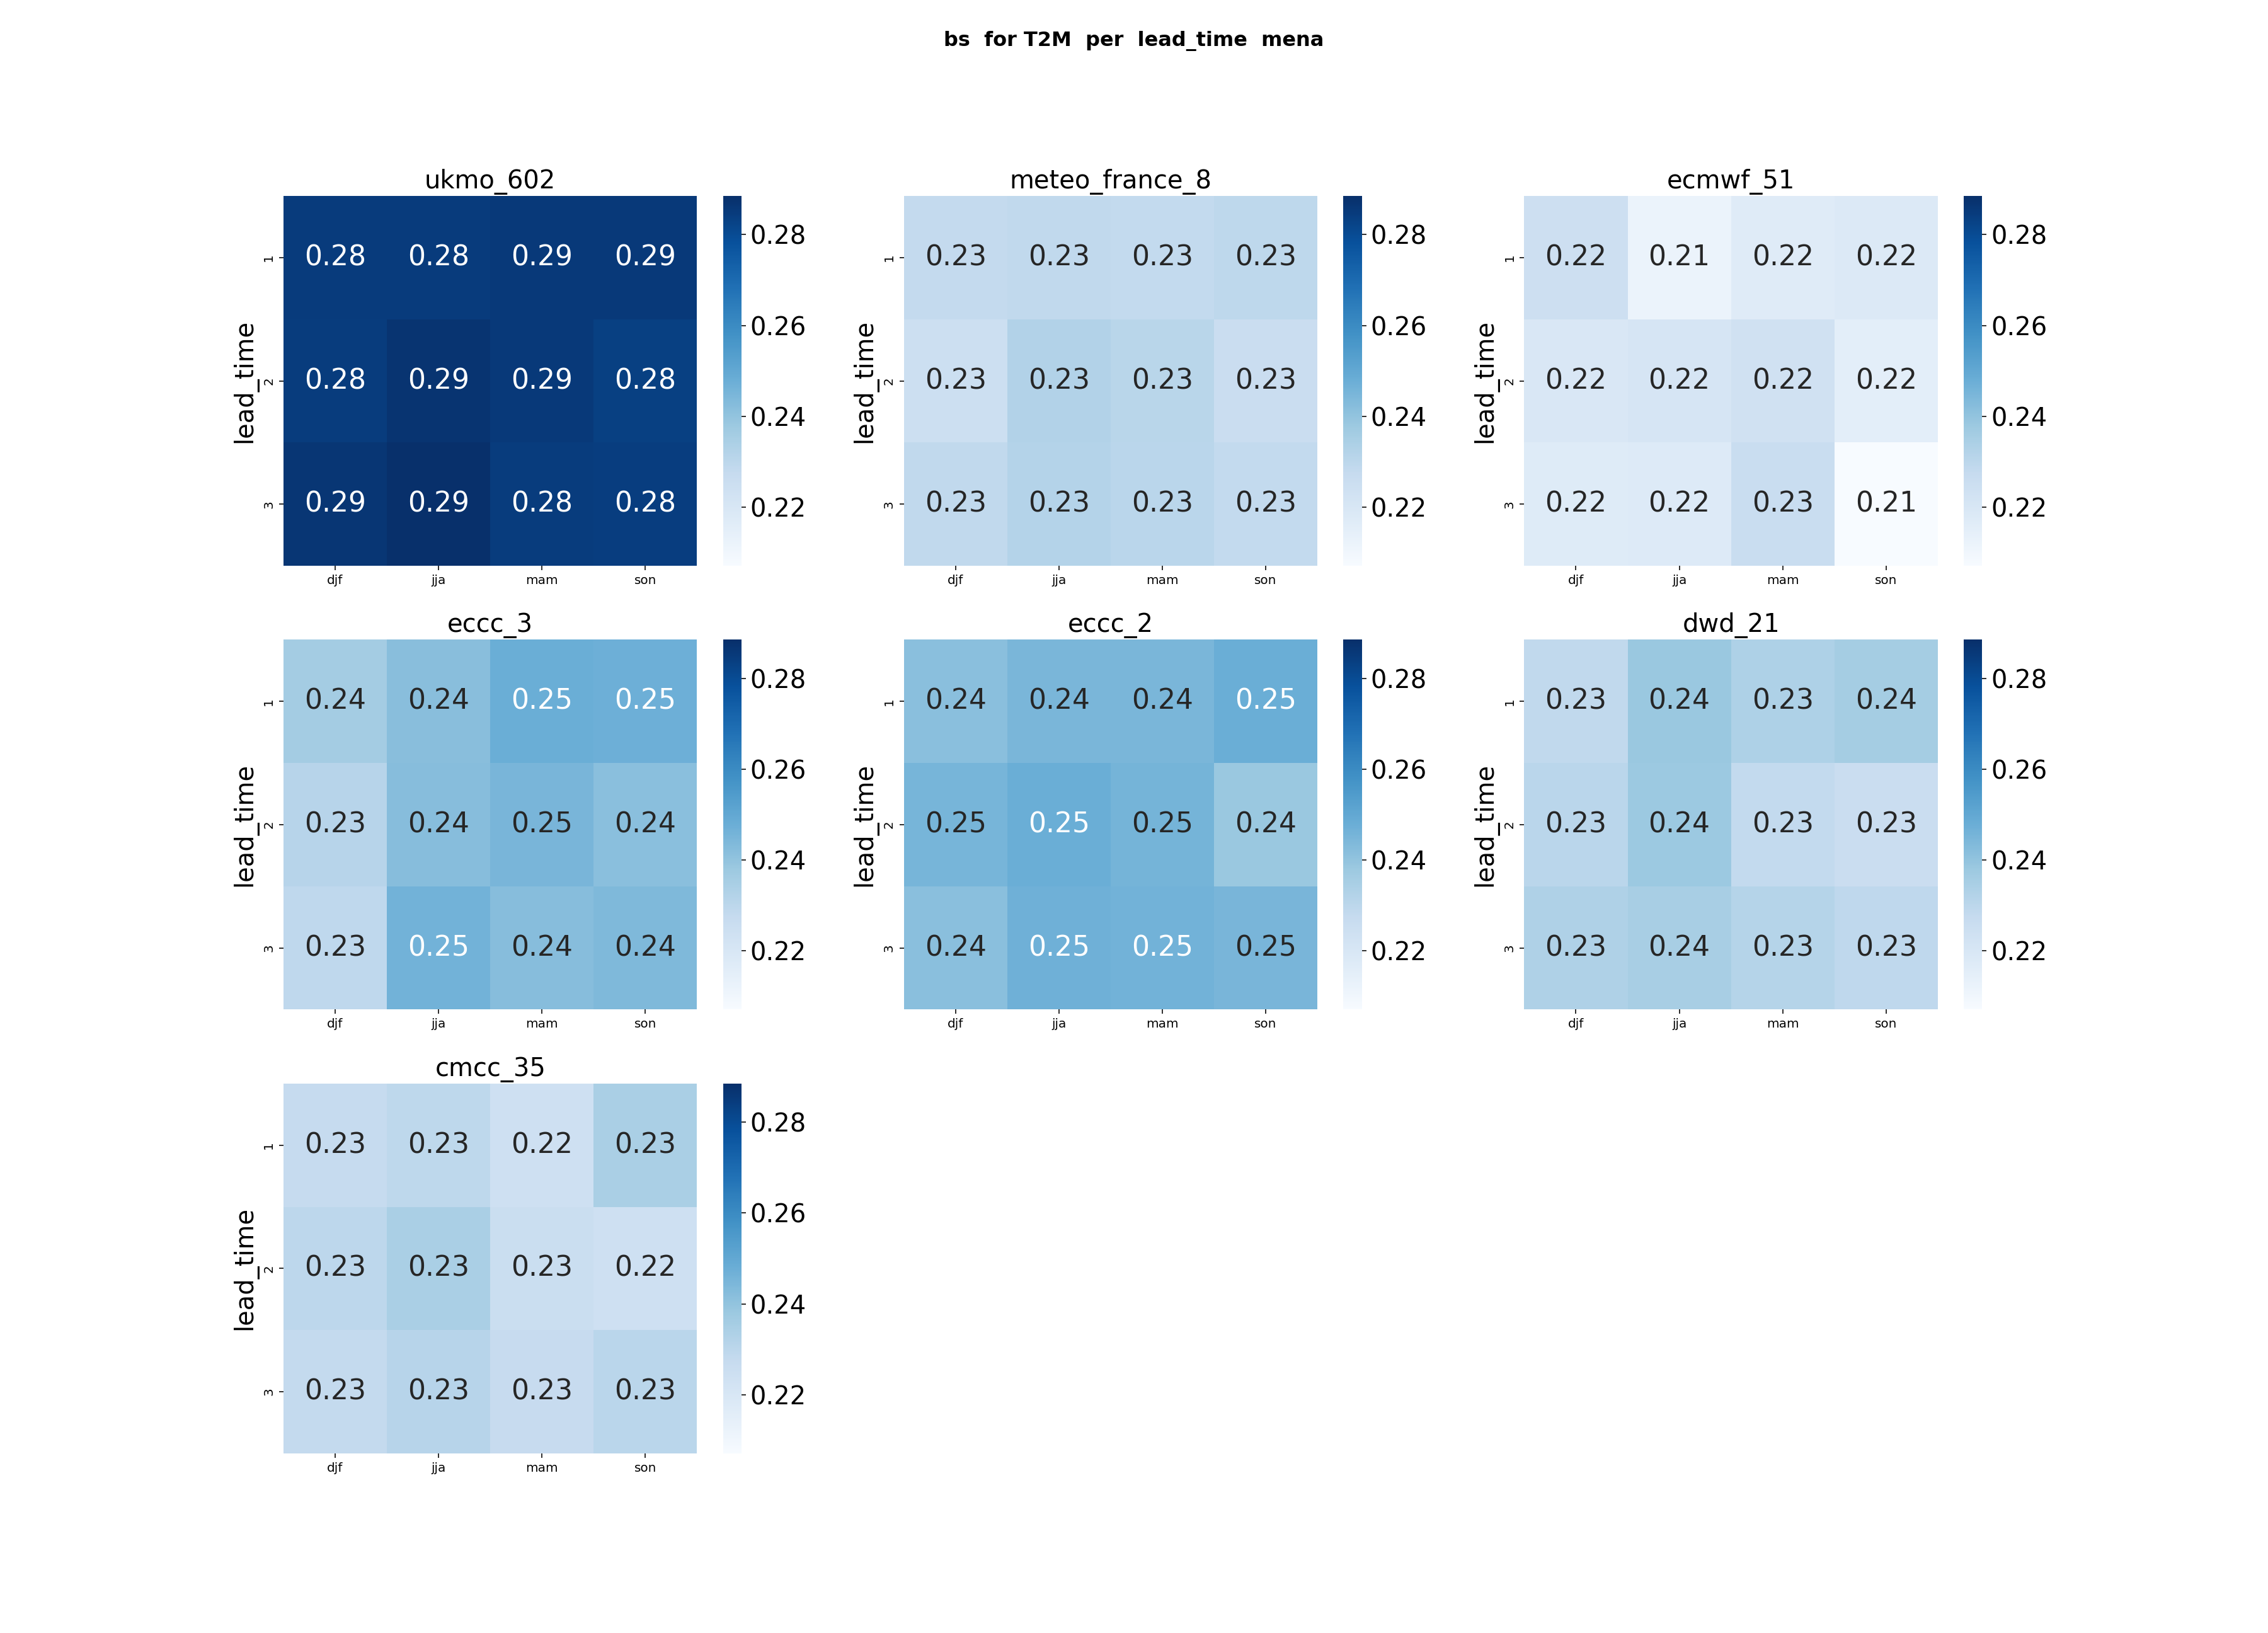
\includegraphics[width=0.8\linewidth]{/home/mohamed/EHTPIII/MODELISATION/Report_25_11/plots/prob/bs/bs_T2M_lead_time_mena.png}
    \caption{Heatmap BS par Par échéance.}
    \label{fig:enter-label}
\end{figure}
\end{frame}


\begin{frame}{Température}
\framesubtitle{Probabiliste - ROC (1 pour un ROC meilleur)}

\begin{figure}
    \centering
    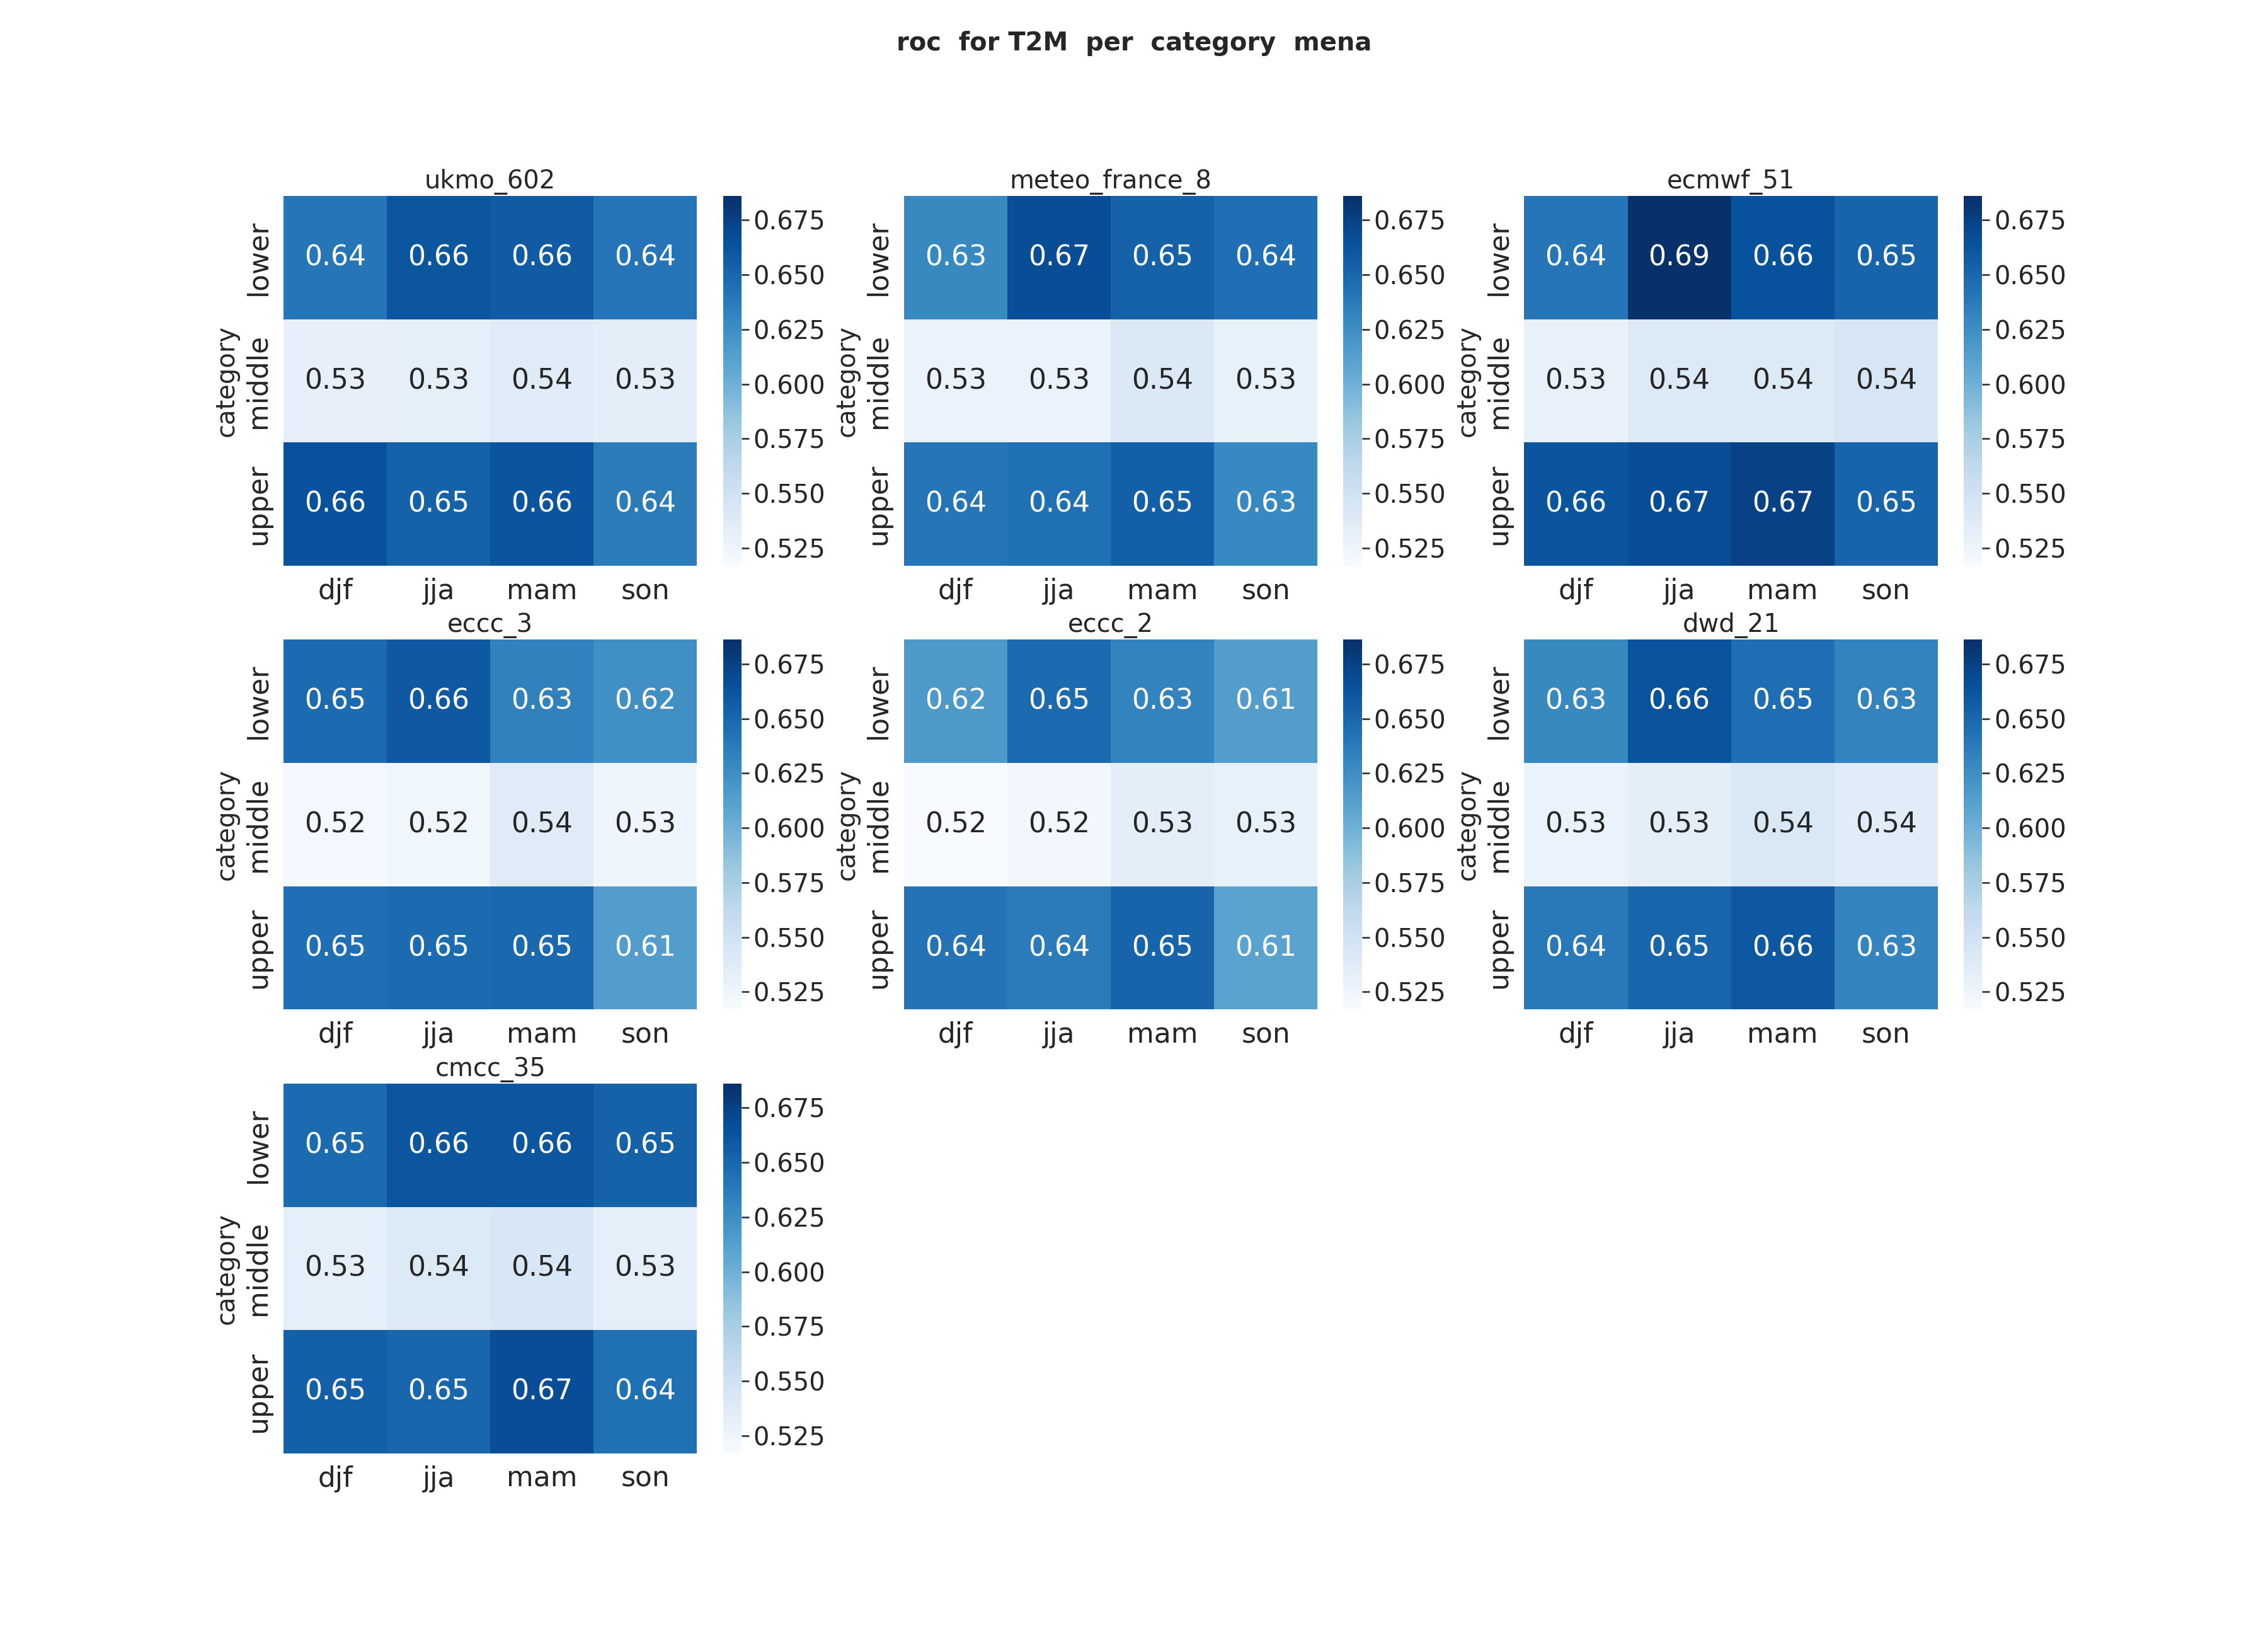
\includegraphics[width=0.8\linewidth]{/home/mohamed/EHTPIII/MODELISATION/Report_25_11/plots/prob/roc/roc_T2M_category_mena.png}
    \caption{Heatmap ROC par Catégorie.  }
    \label{fig:enter-label}
\end{figure}
\end{frame}


\begin{frame}{Température}
\framesubtitle{Probabiliste - ROC (1 pour un ROC meilleur)}

\begin{figure}
    \centering
    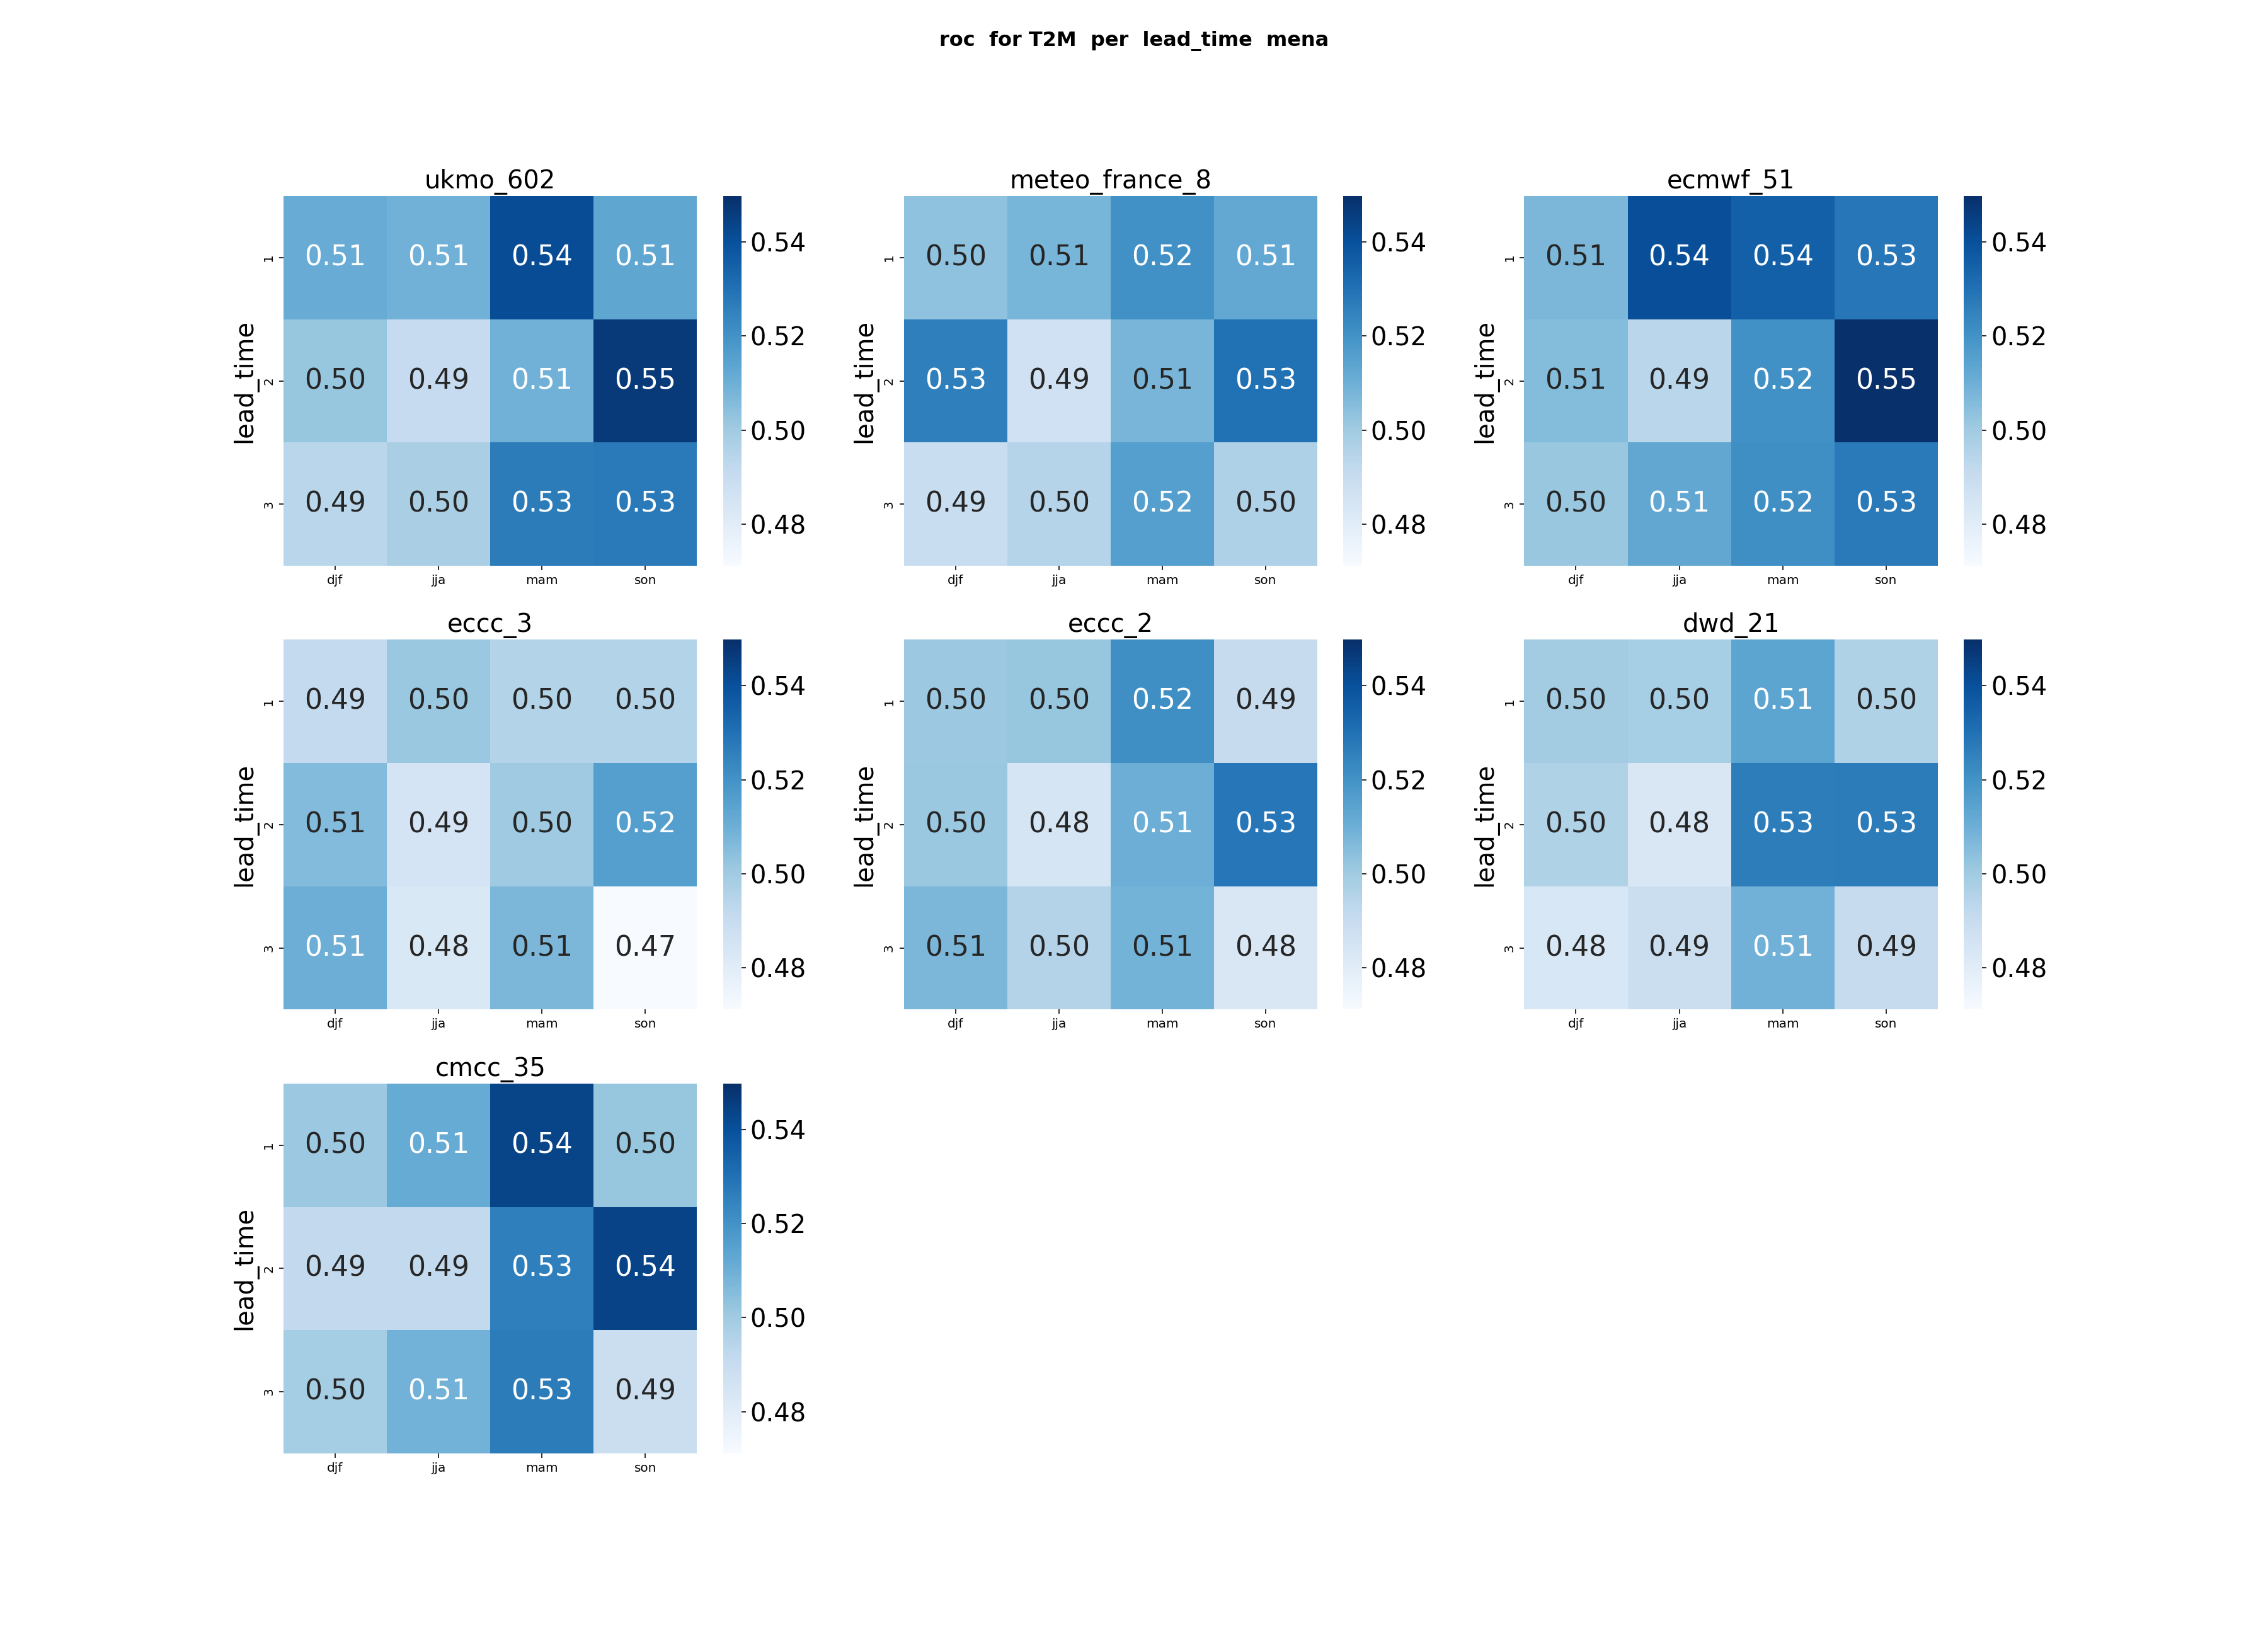
\includegraphics[width=0.8\linewidth]{/home/mohamed/EHTPIII/MODELISATION/Report_25_11/plots/prob/roc/roc_T2M_lead_time_mena.png}
    \caption{Heatmap ROC  Par échéance.}
    \label{fig:enter-label}
\end{figure}
\end{frame}

\begin{frame}{Température}
\framesubtitle{Probabiliste - Reliability (0 pour un score meilleur)}

\begin{figure}
    \centering
    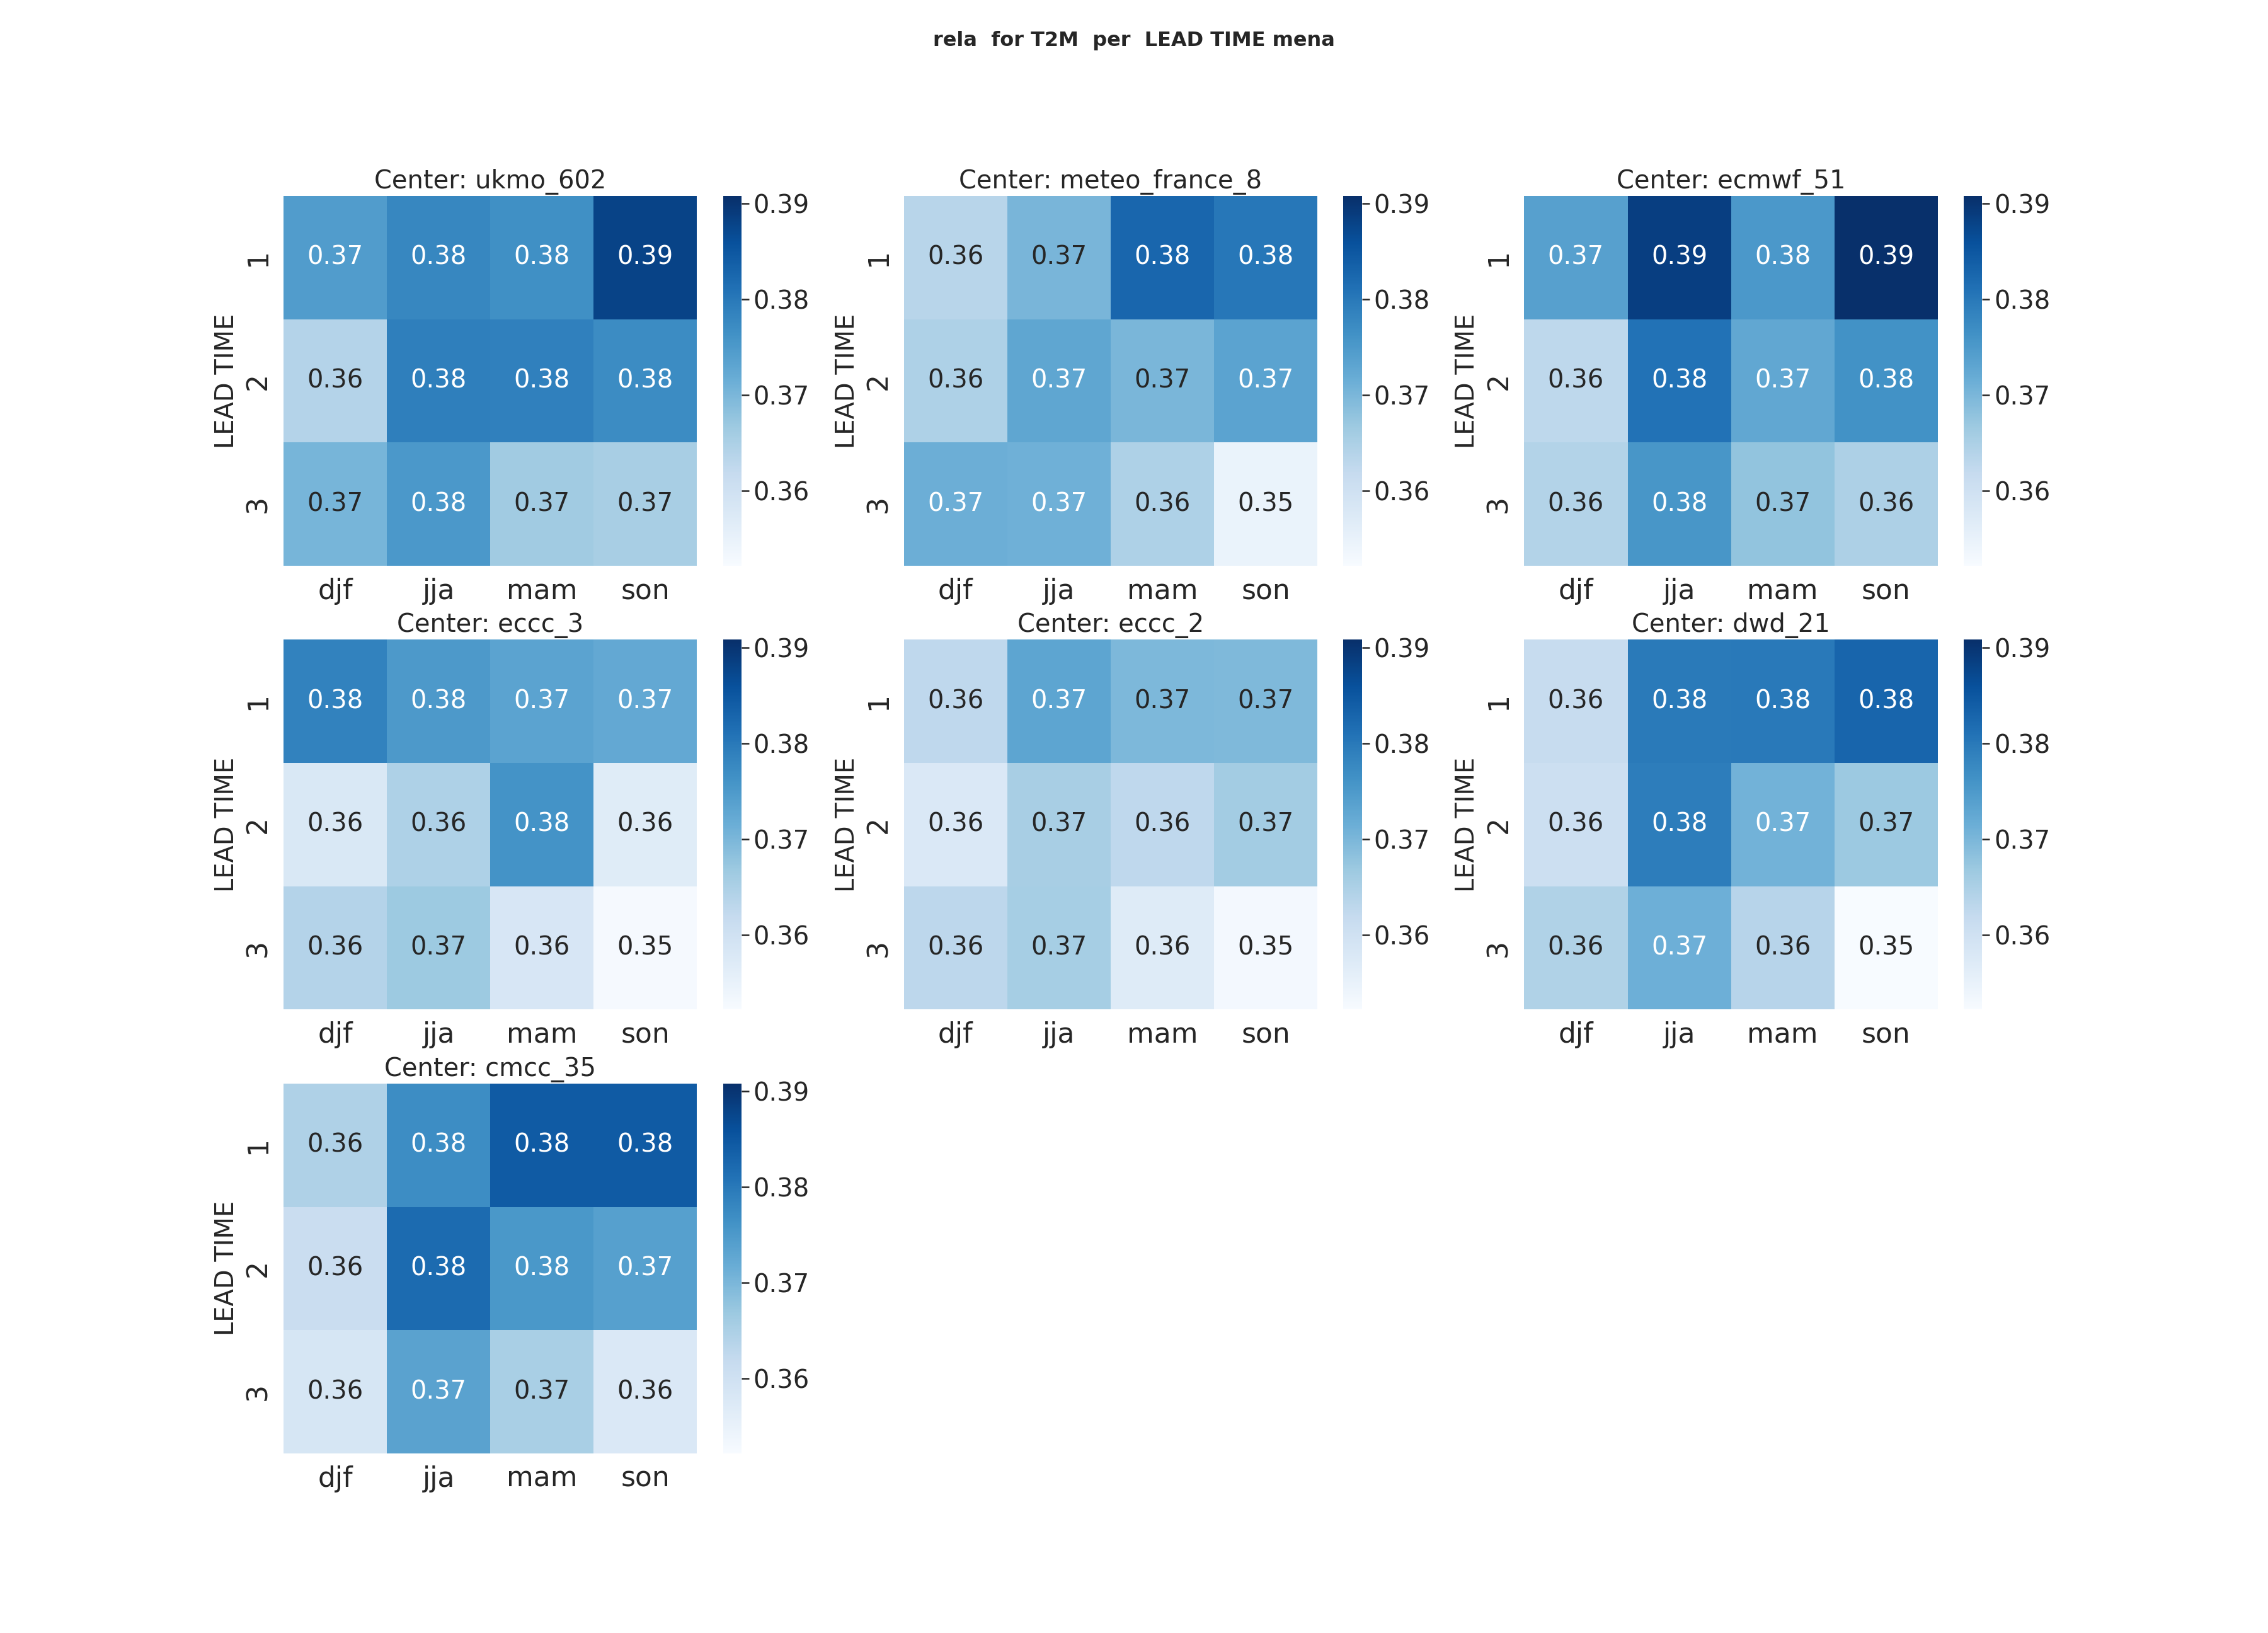
\includegraphics[width=0.6\linewidth]{/home/mohamed/EHTPIII/MODELISATION/Report_25_11/plots/prob/rela/rela_T2M_mena.png}
    \caption{Diagramme de Reliability.}
    \label{fig:enter-label}
\end{figure}
\end{frame}